\documentclass[language=en,12pt]{aghdpl}
\usepackage{hyperref}
\usepackage{svg}
\usepackage{amsmath}

\author{Mateusz Woźniak}
\shortauthor{M. Woźniak}

\titlePL{Operator Kubernetes do harmonogramowania zadań przewidywania konformacji białek na klastrach obliczeniowych w chmurze}
\titleEN{Kubernetes Operator for scheduling protein conformation prediction workloads on cloud computing clusters}

\thesistype{Diploma Thesis}

\supervisor{dr inż. Paweł Skrzyński}

\degreeprogramme{Biomedical Engineering}

\date{2026}

\faculty{Faculty of Electrical Engineering, Automatics, Computer Science and Biomedical Engineering}

\acknowledgements{\small{I would like to dedicate this work to my wonderful
\mbox{Parents \textbf{Joanna and Wojciech Woźniak},} who supported
me throughout my studies, showed me the value of learning, and instilled in me respect for education.
\newline
\newline
For understanding, inspiration, and help, I would like to express my sincere gratitude to my
supervisor \textbf{dr inż. Paweł Skrzyński}. His dedication, professionalism, and valuable advice were invaluable during the implementation of this project.
}}

%TODO(x): W rozdziale "State of the Art", warto było umieścić jedno zdanie podsumowujące kluczowe różnice między opisywanymi narzędziami (np. Foldy vs. Kubefold) przed przejściem do kolejnego podrozdziału.

%TODO: Sekcja 5.2. Challenges mogłaby zawierać więcej refleksji użytkownika – jakie kompromisy musiano podjąć? Jakie elementy sprawiły największy problem koncepcyjnie?

%TODO: Brakuje benchmarków czasu trwania obliczeń w poszczególnych fazach (Aligning, Predicting, Uploading) i jakiejś analizy złożoności obliczeniowej

%TODO(x): Dobrze byłoby pokazać porównanie „before/after” – ile kroków ręcznych wymagałaby instalacja i uruchomienie AlphaFold bez operatora?

%TODO: Warto byłoby rozważyć minimalny rozdział nt. testów – czy komponenty były testowane jednostkowo? Czy działanie operatora było symulowane w testowym klastrze?

%TODO: Przydałoby się więcej odniesień bibliograficznych do istniejących projektów operatorów K8s w naukach biologicznych - brakuje lepszego "osadzenia" prowadzonych badań i ustawienia kontekstu

%TODO: Można by wspomnieć o BioContainers, BioBlend lub Galaxy jako przykładach narzędzi ułatwiających dostęp do bioinformatyki w chmurze.

%TODO: Odniesienie do inicjatywy BioCommons lub ELIXIR mogłoby poszerzyć kontekst aplikacyjny.

\begin{document}

    \titlepages
    \RedefinePlainStyle

    \setcounter{tocdepth}{2}
    \tableofcontents
    \clearpage

    \chapter{Wstęp}


\section{Wprowadzenie}


\section{Motywacja}

Przewidywanie struktury konformacyjnej białek stanowi fundamentalne wyzwanie w naukach biologicznych, mające kluczowe znaczenie między innymi w przemyśle farmaceutycznym, gdzie zrozumienie trójwymiarowej struktury białek jest niezbędne do projektowania nowych leków.
Znajomość struktury przestrzennej białek pozwala zrozumieć ich funkcję biologiczną, mechanizm działania oraz potencjalne interakcje z innymi cząsteczkami, co jest szczególnie istotne w procesie odkrywania nowych substancji terapeutycznych.

Główną motywacją do stworzenia projektu KubeFold było dostrzeżenie istotnej luki technologicznej w obszarze infrastruktury dla przewidywania struktur białkowych.
Choć algorytmy takie jak AlphaFold osiągnęły bezprecedensową dokładność w modelowaniu konformacji białek, ich praktyczne zastosowanie często wymaga specjalistycznej wiedzy z zakresu infrastruktury IT, co stanowi barierę dla wielu badaczy z dziedziny biologii molekularnej czy bioinformatyki.

Dotychczasowe podejścia do uruchamiania AlphaFold często opierały się na ręcznej konfiguracji środowiska obliczeniowego, co wiązało się z wieloma wyzwaniami: począwszy od pobierania i zarządzania gigantycznymi bazami danych białkowych (rzędu terabajtów), przez konfigurację zasobów sprzętowych (w tym wyspecjalizowanych akceleratorów GPU), aż po optymalizację przepływu pracy i zarządzanie artefaktami obliczeń.
Proces ten był czasochłonny, podatny na błędy i wymagał kompetencji z wielu dziedzin jednocześnie.

KubeFold ma na celu przezwyciężenie tych wyzwań poprzez dostarczenie zautomatyzowanej, skalowalnej i łatwej w użyciu platformy, która abstrahuje złożoność infrastrukturalną od użytkownika końcowego.
Dzięki wykorzystaniu technologii konteneryzacji i orkiestracji Kubernetes system zapewnia zautomatyzowane zarządzanie zasobami, elastyczne skalowanie oraz intuicyjny interfejs użytkownika, umożliwiający naukowcom skupienie się na badaniach biologicznych, a nie na aspektach technicznych.


\section{Cele i zakres pracy}

Głównym celem pracy jest zaprojektowanie i implementacja operatora KubeFold dla platformy Kubernetes, który automatyzuje proces uruchamiania obliczeń przewidywania struktury konformacyjnej białek z wykorzystaniem algorytmu AlphaFold.
Realizacja tego celu obejmuje następujące zadania:

\begin{itemize}
    \item Opracowanie architektury operatora Kubernetes, który przede wszystkim:
    \subitem wprowadza zasób \textit{ProteinDatabase} abstrahujący zarządzanie bazami danych białkowych
    \subitem wprowadza zasób \textit{ProteinConformationPrediction} zarządzający faktycznym obliczeniem konformacji białka
    \item Zaprojektowanie i implementacja komponentu do zarządzania bazami danych białkowych, umożliwiającego automatyczne pobieranie i dekompresję plików z danymi
    \item Przygotowanie przykładowego kodu infrastruktury (z ang. \textit{infrastructure as code}), który umożliwia uruchomienie operatora w chmurze Amazon Web Services (AWS) wraz z podpięciem wolumenów \textit{FSx for Lustre}
    \item Wykonanie dokumentacji i instrukcji instalacji operatora w klastrze.
\end{itemize}

Zakres pracy obejmuje pełny cykl wytwarzania oprogramowania: od analizy problemów w istniejących rozwiązaniach, przez projekt architektury, implementację komponentów, aż po weryfikację działania systemu w środowisku Kubernetes.

Projekt nie obejmuje modyfikacji algorytmu AlphaFold, a skupia się na automatyzacji jego uruchamiania w środowisku chmurowym z wykorzystaniem technologii konteneryzacji.


    %! suppress = MissingLabel


\chapter{State of the art}

While the primary focus of this work lies in infrastructure design rather than algorithmic innovation, a brief overview of key prediction algorithms (e.g., AlphaFold) is essential to understand the operational requirements and constraints that the infrastructure must support.


\section{Machine Learning in Protein Structure Prediction}

AlphaFold represents a breakthrough in computational biology, developed by Google DeepMind to predict three--dimensional protein structures with unprecedented accuracy.
This AI system revolutionized the field by achieving near--experimental accuracy in protein structure prediction.

\subsection{Preliminary information}

AlphaFold emerged as the winner of the CASP14 competition in 2020, demonstrating remarkable accuracy in protein structure prediction.
The system leverages deep learning techniques to predict protein structures from amino acid sequences.
AlphaFold 2 represents a significant improvement over previous methods, with a median GDT score exceeding 90 for many targets.
Later AlphaFold 3 extended capabilities to predict protein--protein, protein--nucleic acid, and protein--ligand interactions.
The scientific impact includes accelerating drug discovery, understanding disease mechanisms, and designing novel proteins with specific functions.

\subsection{Algorithm implementation}

AlphaFold implements a novel neural network architecture combining attention mechanisms with structure--based learning.
The algorithm processes protein sequences through multiple specialized neural network blocks.
First, an evolutionary MSA transformer analyzes multiple sequence alignments to capture evolutionary patterns.
Then, a structure module with invariant point attention integrates geometric constraints.
The system iteratively refines predictions through a recycling mechanism that feeds intermediate results back into the network.
Final outputs include 3D atomic coordinates with confidence metrics for each residue.
The implementation balances computational efficiency with prediction accuracy through careful optimization.

\subsection{Program operation overview}

AlphaFold operates in several distinct stages during protein structure prediction, as shown in Figure~\ref{fig:alphafold}.
Initially, it searches sequence databases to build multiple sequence alignments for the target protein.
This first stage requires only CPU resources and involves sequence similarity searches against large databases.
Next, the system processes this data through its neural network architecture to generate initial structure predictions, a stage that exclusively requires GPU resources for efficient tensor operations.
The prediction undergoes multiple refinement cycles, where each iteration improves model quality.
AlphaFold produces five candidate models with associated confidence scores (pLDDT). The deployment involves containerized environments for reproducibility across computing platforms.
Output formats include PDB files for 3D coordinates and additional files containing confidence metrics and model parameters.

\begin{figure}[htbp]
    \centering
    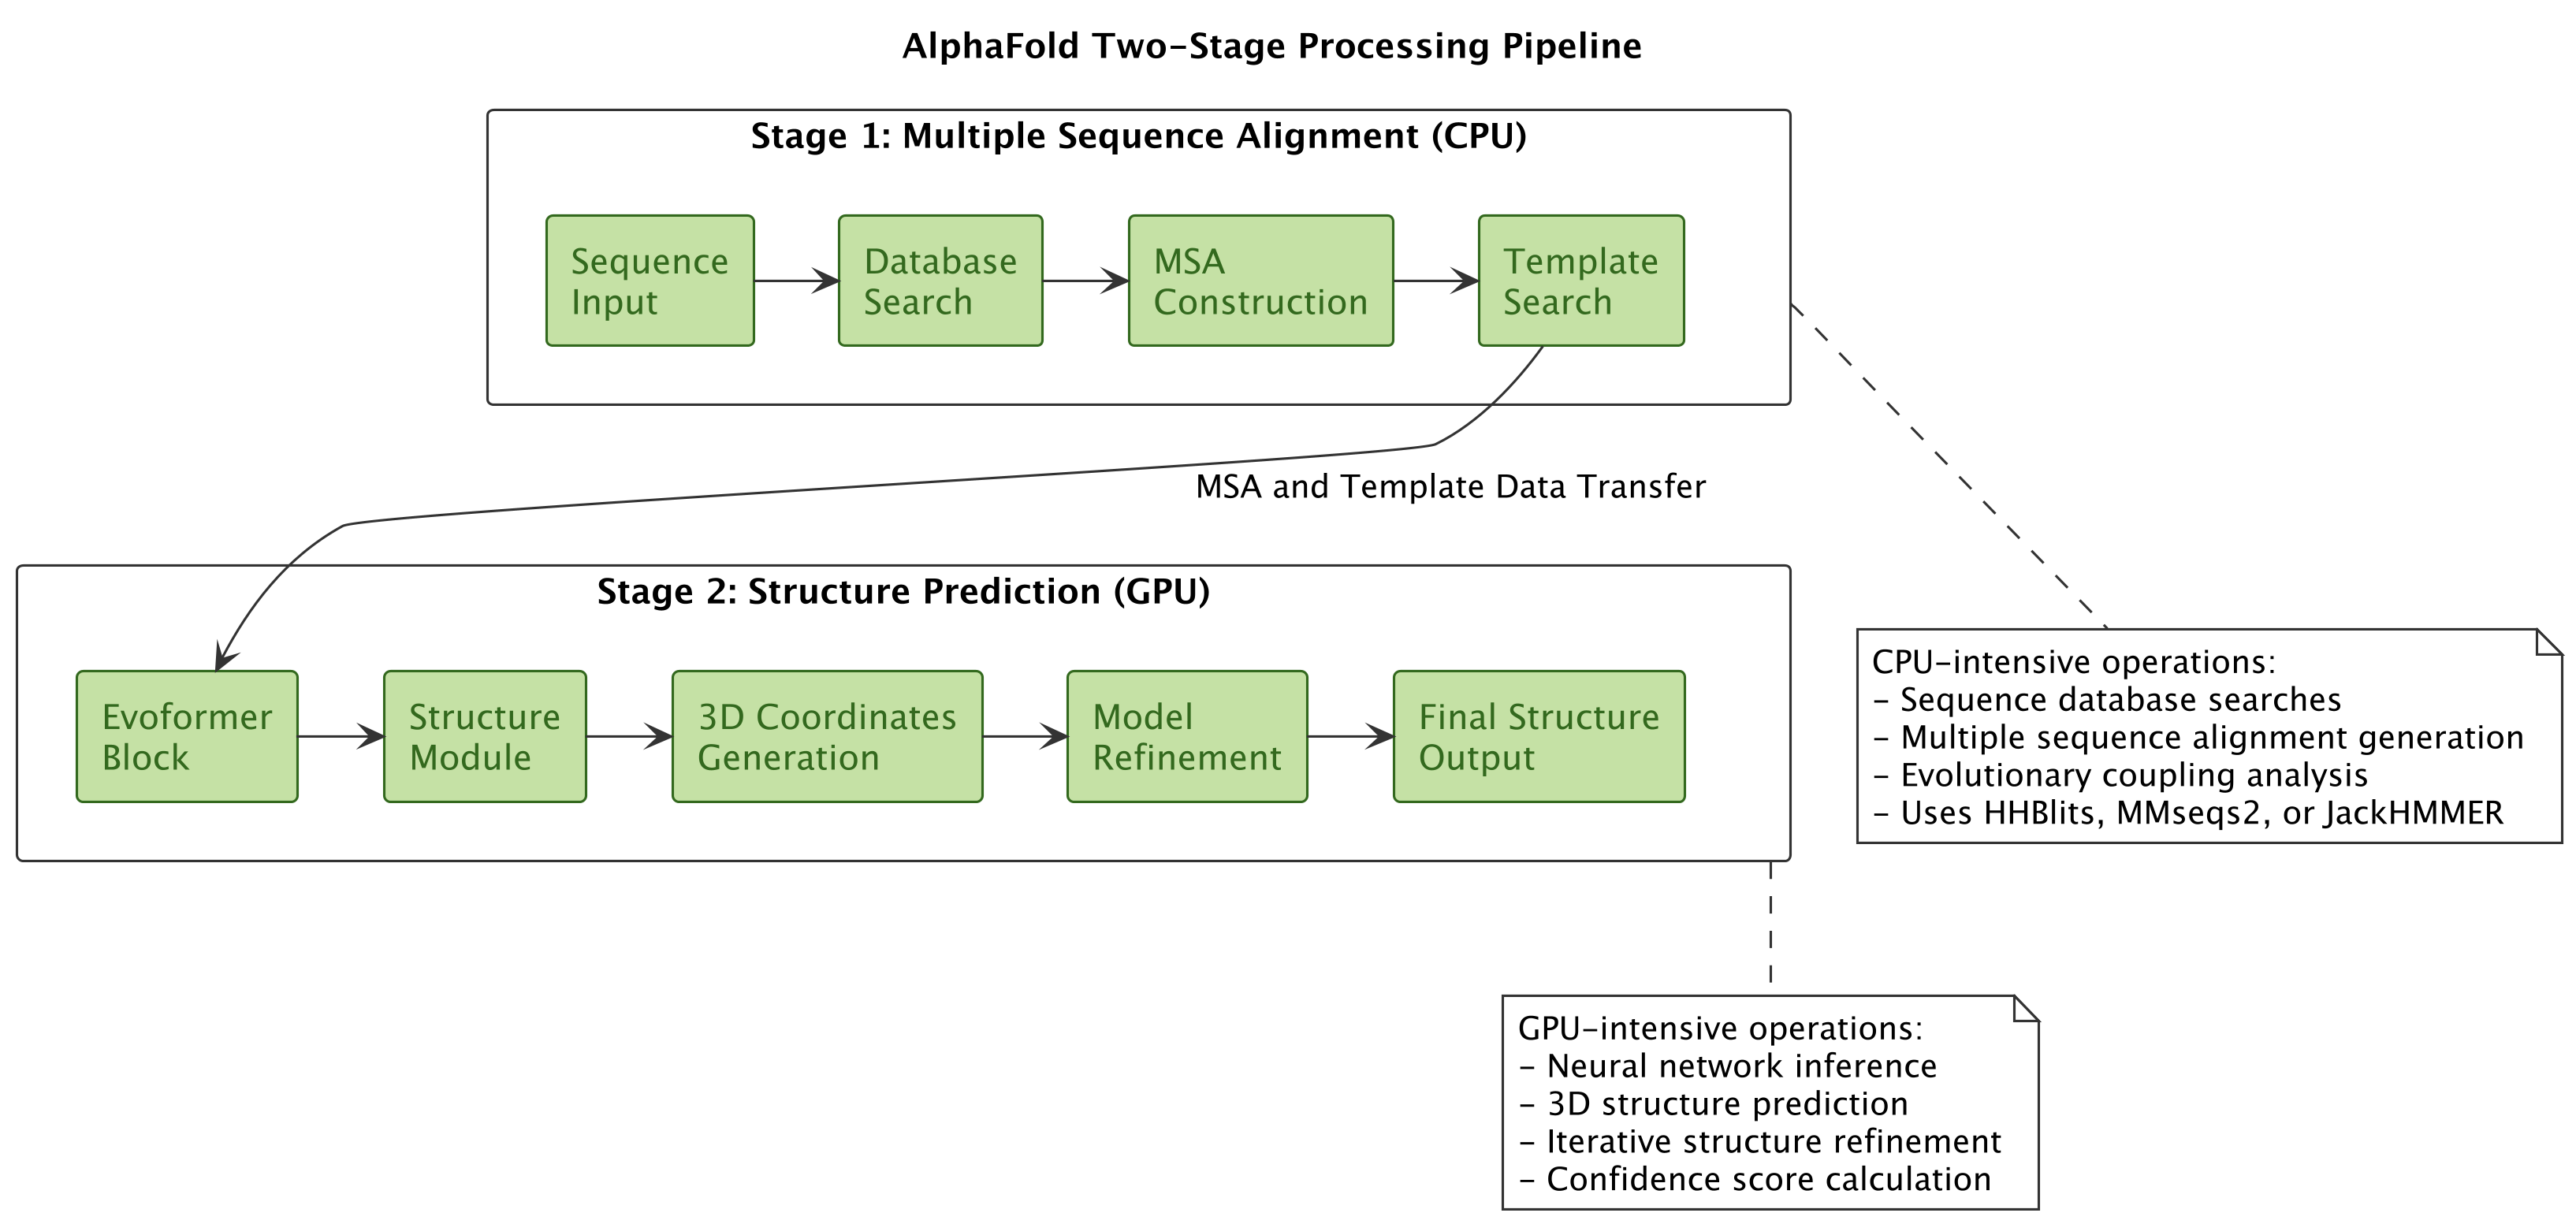
\includegraphics[width=\textwidth]{images/alphafold}
    \caption{AlphaFold 3 computation stages}
    \label{fig:alphafold}
\end{figure}

\subsection{Required computational resources}

AlphaFold demands substantial computational resources for effective operation.
The system requires high--performance GPUs, preferably NVIDIA A100 or similar, with at least 16GB VRAM. Memory requirements range from 16GB for small proteins to 64GB+ for large complexes.
Storage needs include approximately 2TB for reference databases and additional space for output models.
Prediction time varies significantly with protein size and complexity, ranging from 30 minutes for small proteins to several hours for complex structures.
Cloud--based deployments typically cost between $10--$100 per prediction depending on computational requirements.
The high resource demands make AlphaFold particularly suitable for execution in specialized computing environments with access to dedicated hardware accelerators.


\section{Computational clusters in a cloud environment}

\subsection{Kubernetes platform}

Kubernetes is an open--source container orchestration software that automates the deployment, scaling, and management of applications~\cite{kubernetes, container_orchestration}.
It is currently the main solution in the area of computational cluster management.
Kubernetes originates from Google's internal project called Borg, which was released as an open--source project in 2014.

The main goal of Kubernetes is to provide a platform for running applications in a distributed environment.
The system enables automatic management of computational resources in a heterogeneous hardware environment, encompassing different processor architectures and dedicated computational accelerators.
Kubernetes eliminates many manual processes related to deploying and scaling containerized applications.
All cluster components are controlled declaratively.

The Kubernetes architecture is based on a master--worker node model.
The main control component (control plane) manages worker nodes, on which actual applications are run in containers.
Each Kubernetes cluster consists of at least one master node and many worker nodes.
This architecture provides high availability and fault tolerance.

The resource model in Kubernetes is declarative.
Pod is the basic deployment unit in Kubernetes, representing one or more containers that share resources and are always run on the same cluster node.
After loading a configuration file in YAML format, Kubernetes will strive to bring the actual state of the cluster to the state declared in the configuration.
An example of a \texttt{Deployment} resource declaration shown in listing~\ref{lst:kube-deployment} contains comments explaining key elements:

\begin{lstlisting}[language=yaml,caption={Example Deployment declaration in Kubernetes},label={lst:kube-deployment}]
apiVersion: apps/v1
# Kubernetes resource type
kind: Deployment 
metadata:
  name: nginx-deployment
  labels:
    app: nginx
spec:
  # Number of replicas (copies) of the pod to run
  replicas: 3
  # Selector specifying which pods belong to the deployment
  selector:
    matchLabels:
      app: nginx
  # Template defining pod specification
  template:
    metadata:
      labels:
        app: nginx
    spec:
      containers:
      # Container definition to run
      - name: nginx
        image: nginx:1.14.2
        ports:
        - containerPort: 80  # Port to listen on in the container
\end{lstlisting}

Kubernetes introduces an abstraction of the infrastructure layer.
This allows applications to be moved between different cloud providers without modifying code.
The platform supports various runtime environments, from local clusters, through private clouds, to major public cloud providers.

Key capabilities of Kubernetes include:
\begin{itemize}
    \item Automatic application recovery in case of failure,
    \item Load balancing and network traffic distribution,
    \item Automatic horizontal scaling of applications based on a load,
    \item Configuration and secrets management,
    \item Persistent storage management,
    \item Batch execution for batch jobs and computation scheduling.
\end{itemize}

Kubernetes was designed as an extensible platform.
It allows creating custom controllers and operators tailored to specific needs.
This extensibility is key for the KubeFold project, which uses these mechanisms to orchestrate complex protein conformation prediction tasks.

\subsection{Architecture and components of a Kubernetes cluster}

A Kubernetes cluster consists of two main parts: the Control Plane and Worker Nodes, as shown in Figure~\ref{fig:kubernetes-architecture}.
This architecture provides the foundation for running containerized applications like AlphaFold in a distributed environment~\cite{kubernetes}.

The Control Plane contains components that manage the entire cluster and store its state:
\begin{itemize}
    \item \textbf{kube--api--server} -- the access point to the cluster, handling all API requests and providing the interface for communication,
    \item \textbf{etcd} -- a key--value database storing the entire cluster state, serving as the persistent storage for all cluster configuration,
    \item \textbf{kube--scheduler} -- responsible for assigning workloads to nodes based on resource requirements and constraints,
    \item \textbf{kube--controller--manager} -- supervises the cluster state, ensuring it matches the declared configuration by running controller processes,
    \item \textbf{cloud--controller--manager} -- integrates the cluster with cloud provider infrastructure, managing cloud--specific resources.
\end{itemize}

Worker Nodes run actual workloads in the form of containers.
Each worker node contains:
\begin{itemize}
    \item \textbf{kubelet} -- an agent managing containers on the node, ensuring they are running and healthy,
    \item \textbf{kube--proxy} -- handling network traffic and ensuring routing between services across the cluster,
    \item \textbf{Pods} -- the basic deployment units containing one or more containers that share networking and storage resources.
\end{itemize}

As described earlier in the Kubernetes Platform section, the system defines higher--level abstractions such as \texttt{Deployment} or \texttt{StatefulSet}.
These enable declarative application management through configuration files in YAML format.
The Service resource provides a stable access point to a group of Pods, abstracting the underlying infrastructure changes.

The cluster uses a plugin system to extend functionality.
This includes storage, network, or monitoring drivers.
Particularly important for the KubeFold project are Custom Resource Definitions, which allow adding custom resource types as discussed in the Cluster Operator section.

The Kubernetes architecture ensures high availability, scalability, and fault tolerance required for computational tasks like protein structure prediction.
Components can be duplicated across nodes to prevent single points of failure.
The system automatically responds to failures by restarting and relocating applications, maintaining the desired state of the cluster.

\begin{figure}[htbp]
    \centering
    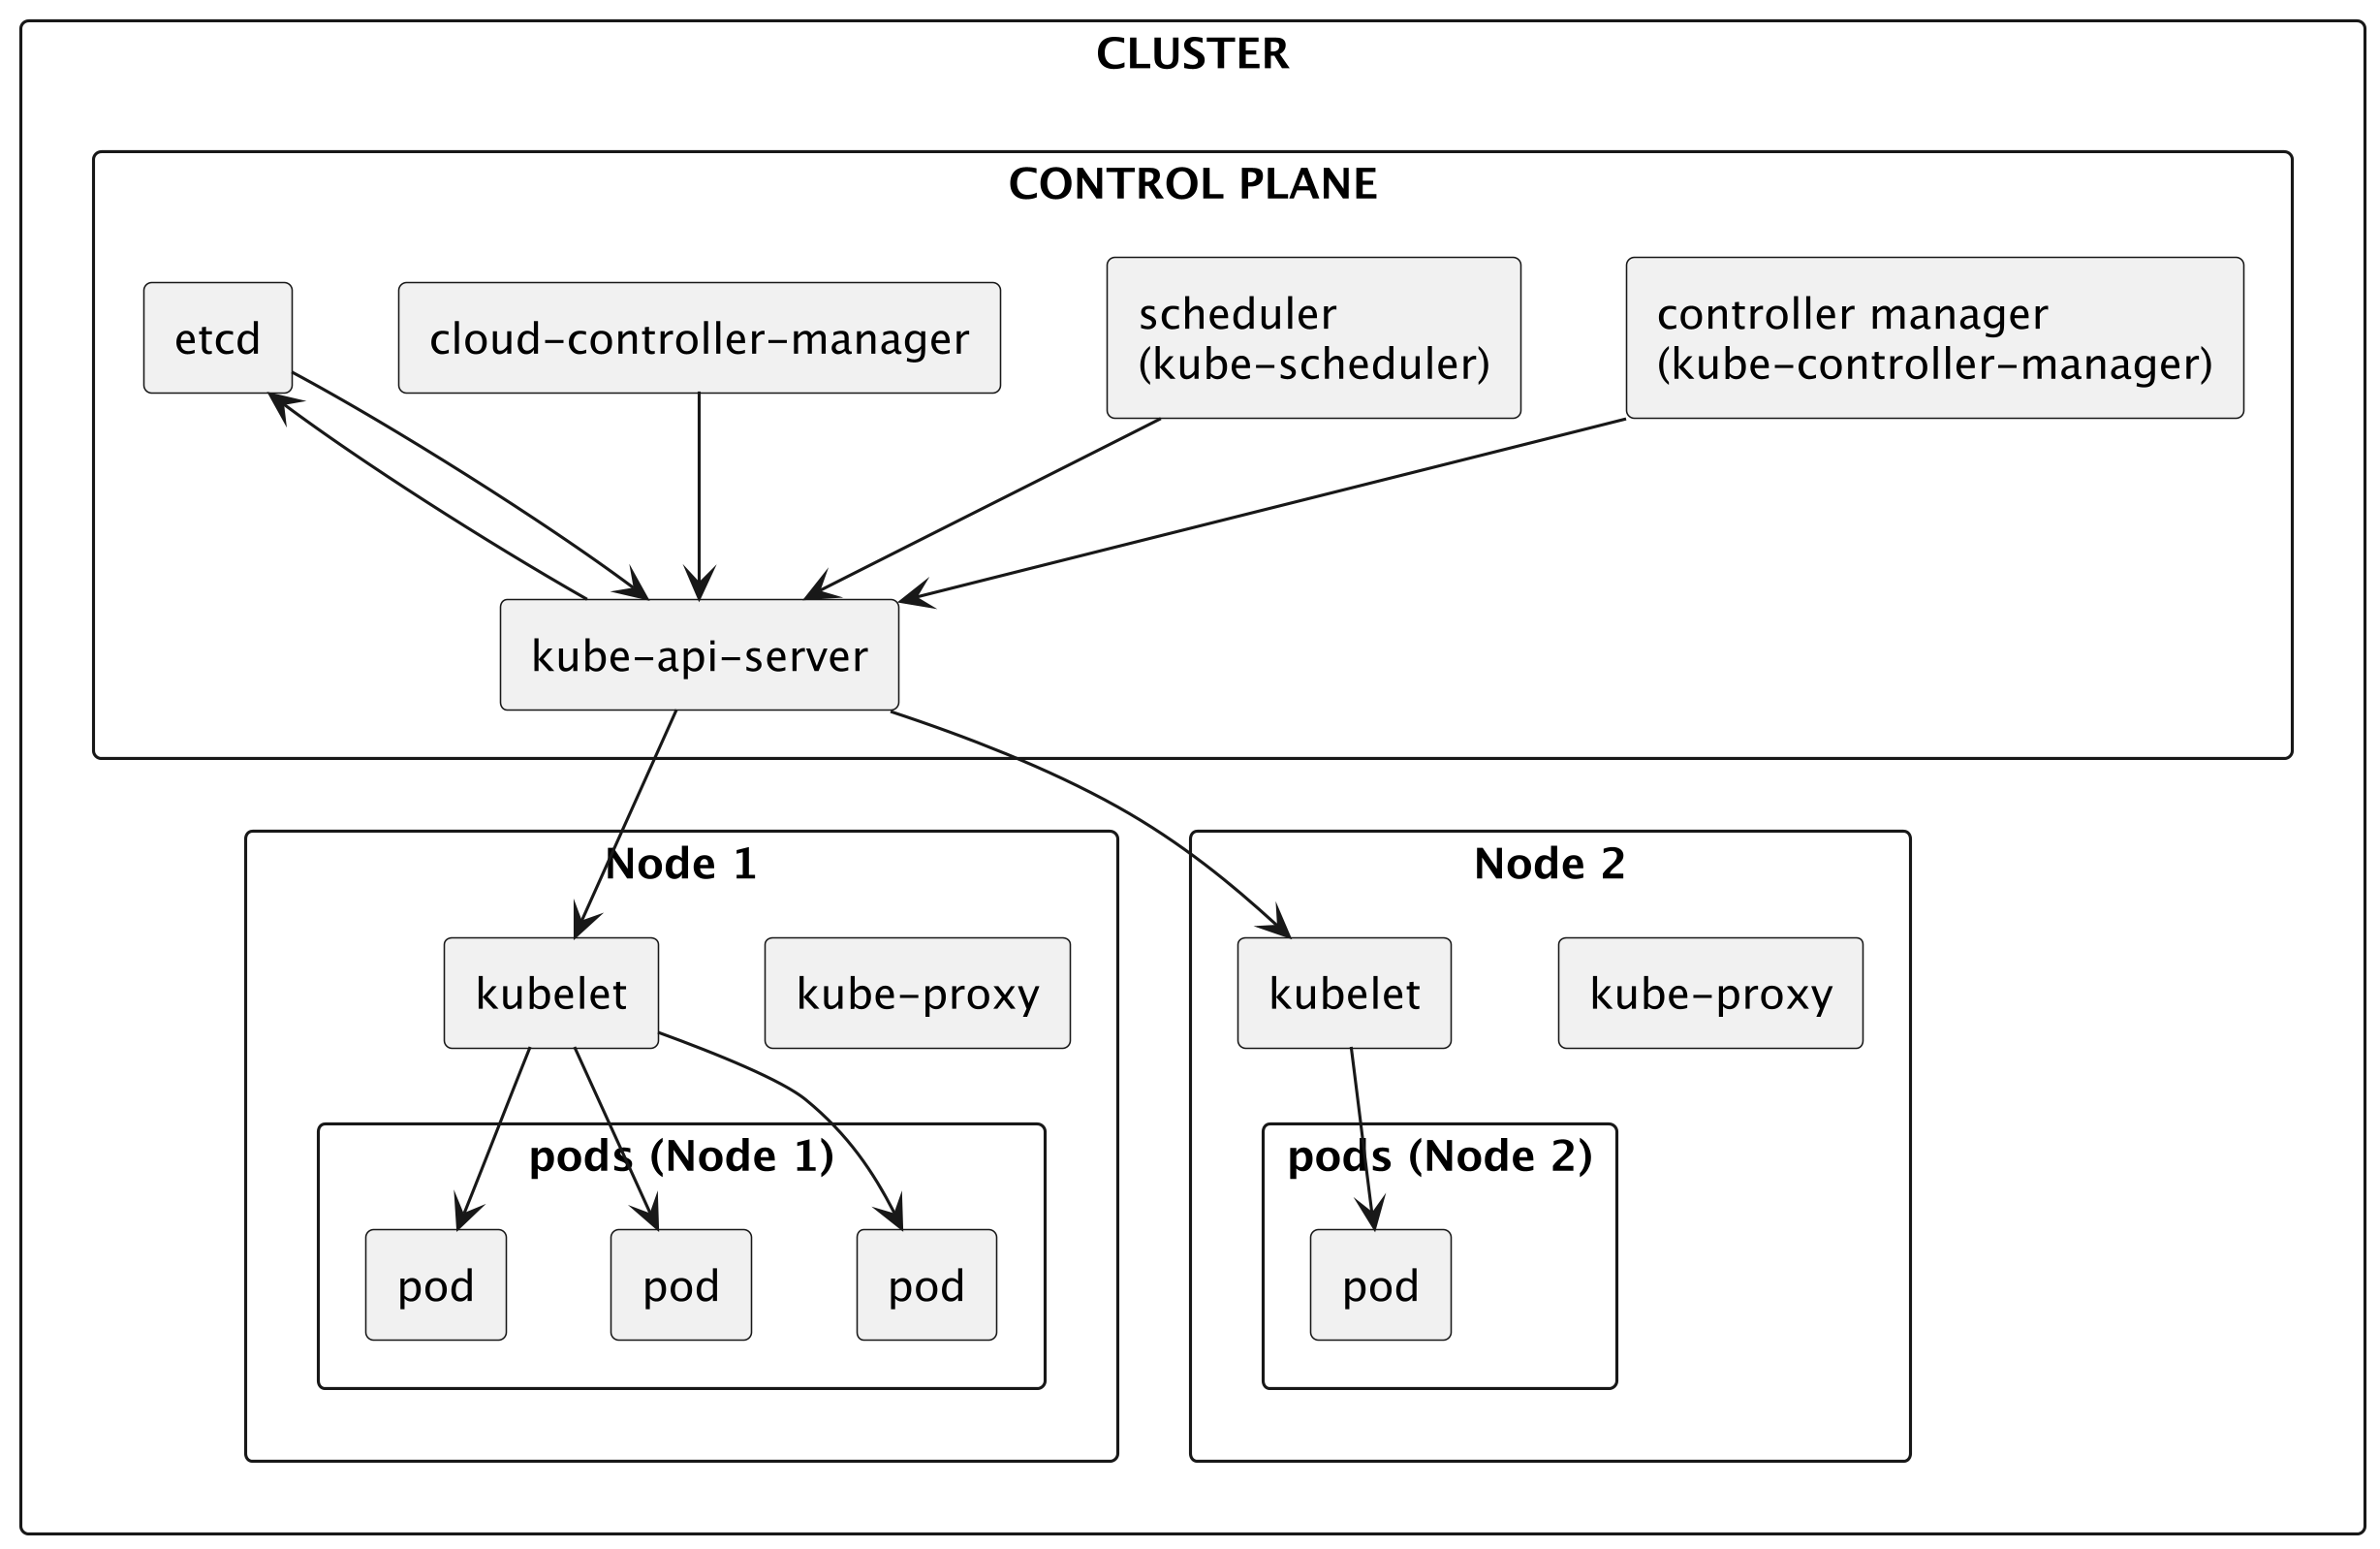
\includegraphics[width=\textwidth]{images/kubernetes}
    \caption{Kubernetes cluster architecture showing Control Plane components (kube--api--server, etcd, scheduler, controller manager, cloud--controller--manager) and Worker Nodes containing kubelet, kube--proxy, and pods. The diagram illustrates the communication between the control plane and worker nodes, with the cloud provider API interface for external resource management.}
    \label{fig:kubernetes-architecture}
\end{figure}

\subsection{Available resources in the computational cluster}
Kubernetes platform defines basic resource types used to manage applications in a computational cluster.
Each resource type serves a specific role and can be configured by administrators and applications.

\subsubsection{Pod}
Pod is the basic deployment unit in a Kubernetes cluster.
It represents a process executing an application along with its execution context.
A Pod contains one or more containers sharing network space and storage resources.
Listing~\ref{lst:pod-example} shows an example definition of a Pod with an application server and an attached data volume.

\begin{lstlisting}[language=yaml,caption={Example Pod definition},label={lst:pod-example}]
apiVersion: v1
kind: Pod
metadata:
  name: web-server
  labels:
    app: web
spec:
  containers:
  - name: nginx
    image: nginx:latest
    resources:
      limits:
        memory: "128Mi"
        cpu: "500m"
    volumeMounts:
    - name: www-data
      mountPath: /usr/share/nginx/html
  volumes:
  - name: www-data
    persistentVolumeClaim:
      claimName: web-content
\end{lstlisting}

\subsubsection{Job}
Job represents a computational task with a finite execution time.
This resource guarantees successful execution of a specified number of Pods.
In case of a computational node failure, the Job automatically creates a new Pod instance.
Listing~\ref{lst:job-example} shows an example of a Job performing batch file conversion.

\begin{lstlisting}[language=yaml,caption={Example Job definition},label={lst:job-example}]
apiVersion: batch/v1
kind: Job
metadata:
  name: batch-convert
spec:
  template:
    spec:
      containers:
      - name: converter
        image: imagemagick:latest
        command: ["convert"]
        args: ["*.jpg", "-resize", "800x600", "output/"]
      restartPolicy: Never
  backoffLimit: 4
\end{lstlisting}

\subsubsection{PersistentVolume}
PersistentVolume defines a persistent storage volume in the cluster.
It is independent of the Pod lifecycle and stores data that must survive cluster restarts.
Listing~\ref{lst:pv-example} shows the definition of a volume using the NFS file system.

\begin{lstlisting}[language=yaml,caption={Example PersistentVolume definition},label={lst:pv-example}]
apiVersion: v1
kind: PersistentVolume
metadata:
  name: nfs-volume
spec:
  capacity:
    storage: 100Gi
  accessModes:
    - ReadWriteMany
  persistentVolumeReclaimPolicy: Retain
  nfs:
    server: nfs-server.example.com
    path: "/shared"
\end{lstlisting}

\subsubsection{PersistentVolumeClaim}
PersistentVolumeClaim is a request for allocation of storage resources~\cite{k8s_persistent_volumes}.
It defines requirements regarding the size and access mode for the volume.
Listing~\ref{lst:pvc-example} shows an example request for creating a 10GB volume.

\begin{lstlisting}[language=yaml,caption={Example PersistentVolumeClaim definition},label={lst:pvc-example}]
apiVersion: v1
kind: PersistentVolumeClaim
metadata:
  name: web-content
spec:
  accessModes:
    - ReadWriteMany
  resources:
    requests:
      storage: 10Gi
  storageClassName: standard
\end{lstlisting}

\subsubsection{StorageClass}
StorageClass describes a storage class available in the cluster.
It defines the provider and configuration parameters for volumes.
Listing~\ref{lst:sc-example} shows the definition of a standard storage class for SSD disks.

\begin{lstlisting}[language=yaml,caption={Example StorageClass definition},label={lst:sc-example}]
apiVersion: storage.k8s.io/v1
kind: StorageClass
metadata:
  name: fast-storage
provisioner: kubernetes.io/aws-ebs
parameters:
  type: gp3
  iopsPerGB: "5000"
  encrypted: "true"
reclaimPolicy: Delete
allowVolumeExpansion: true
\end{lstlisting}

\subsection{Volume allocation mechanism}
Kubernetes uses a complex mechanism for dynamic allocation of storage resources.
When an application creates a PersistentVolumeClaim, the system checks the storage class (StorageClass) declared in it.
Based on this, it activates the appropriate driver that creates a physical volume in the infrastructure.
The newly created PersistentVolume is then automatically linked to the claim.
Thanks to this mechanism, a cluster administrator can define different storage classes, and users can use them without knowing the technical details of the infrastructure.
The system guarantees that the volume will exist as long as the claim associated with it exists.
After deleting a PersistentVolumeClaim, the fate of the volume depends on the defined reclaim policy -- it can be automatically deleted or preserved for reuse.

\subsection{Kubernetes clusters in the cloud}

Kubernetes clusters in a cloud environment represent a natural evolution of computational platforms.
The cloud offers dynamic resource allocation and integration with services such as data stores or monitoring systems.
Geographic distribution ensures high availability, and automatic backup mechanisms protect against data loss.
Advanced access control systems guarantee the security of data and applications.

Public cloud providers offer managed Kubernetes services that automate most administrative tasks.
This includes cluster creation and configuration, component updates, and infrastructure state monitoring.
Thanks to this, teams can focus on application development instead of infrastructure maintenance.

\subsection{Managed Kubernetes service in Amazon Web Services}\label{subsec:aws-eks}

Amazon Elastic Kubernetes Service (EKS) is a comprehensive solution for running Kubernetes clusters in the AWS cloud~\cite{amazon_eks}.
The service automatically manages control node updates, certificates, and network configuration.
Integration with AWS services simplifies creating solutions using data stores or notification systems.

In the context of the KubeFold project, access to instances equipped with graphics cards and integration with the FSx for Lustre file system are of key importance.
EKS enables automatic scaling of the node group depending on demand, which translates into cost optimization.

Using Kubernetes clusters in the cloud brings significant benefits for computational projects.
Elimination of costs for maintaining own infrastructure and access to specialized hardware without the need to purchase allow for flexible budget management.
The billing model based on actual resource consumption works particularly well in the case of computations with varying intensity, such as protein conformation prediction.
Automatic recovery mechanisms after failure and global availability ensure reliability and high--quality services.
This combination of features makes cloud Kubernetes clusters an optimal environment for modern scientific applications.

\subsection{Lustre volumes}\label{subsec:lustre-volumes}

Lustre is a distributed file system, created by Cluster File Systems in 2003~\cite{lustre_fs}.
This system was designed for high--performance computing clusters.
Currently, the development of Lustre is managed by the OpenSFS (Open Scalable File Systems) organization.

The Lustre file system consists of several main components, as shown in Figure~\ref{fig:lustre-arch}:
\begin{itemize}
    \item Metadata servers (MDS) -- store information about the file system structure, directories, and permissions,
    \item Object storage servers (OSS) -- responsible for storing actual data and handling input/output operations,
    \item Clients -- nodes that mount the file system and use it,
    \item Metadata target devices (MDT) -- store metadata on block devices,
    \item Object storage targets (OST) -- store file data on block devices.
\end{itemize}

\begin{figure}[htbp]
    \centering
    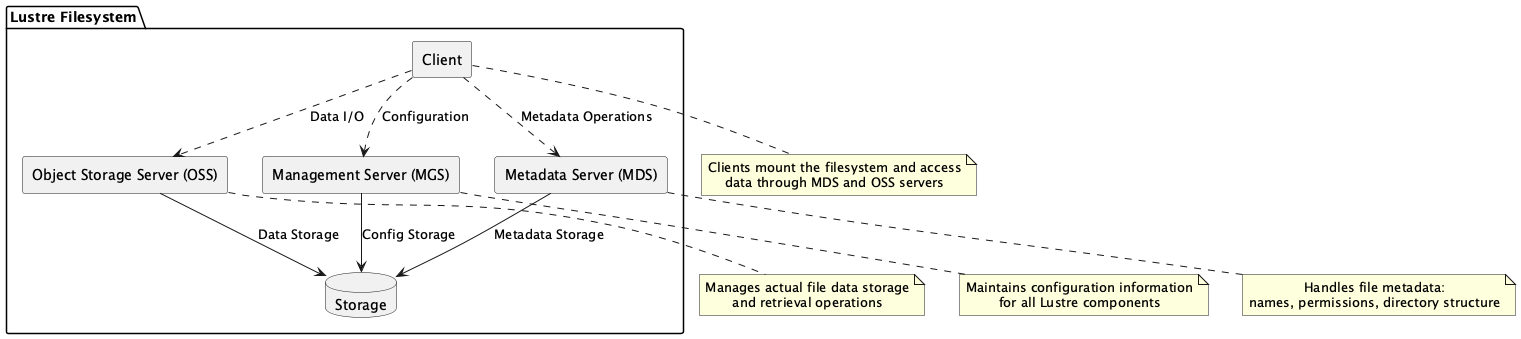
\includegraphics[width=\textwidth]{images/lustre}
    \caption{Lustre distributed file system architecture showing the relationships between metadata servers, object storage servers, and clients.}
    \label{fig:lustre-arch}
\end{figure}

The Lustre architecture is based on the separation of metadata from actual data.
Metadata servers deal exclusively with operations on directory structure and permissions.
Object servers handle operations on the file data itself.
Such separation allows for optimization of both types of operations independently.

Lustre ensures very high performance through parallel input/output operations.
The system enables simultaneous access to the same files from multiple cluster nodes.
A single Lustre file system can serve tens of thousands of clients simultaneously.
The system's throughput scales linearly with the addition of more object servers.

Main features of the Lustre file system:
\begin{itemize}
    \item High scalability -- ability to handle petabytes of data and thousands of nodes,
    \item High throughput -- ability to achieve throughput in the terabit per second range,
    \item Cache coherence -- guarantee of data consistency between all clients,
    \item Fault tolerance -- ability to work despite failure of individual components,
    \item Support for multiple access protocols -- POSIX, MPI--IO, HDFS\@.
\end{itemize}

In the KubeFold project, Lustre is a key component for storing protein databases.
Its architecture ensures high throughput and low latency when accessing data.
The system allows simultaneous access to files from multiple cluster nodes performing calculations.
This makes it possible to parallel process data by multiple instances of the AlphaFold algorithm.

Lustre is widely used in computing centers around the world.
It is used in supercomputers from the TOP500 list.
The system works particularly well in scientific computing, where processing huge datasets is required.
Examples of applications include physical simulations, climate modeling, and genomic calculations.

\subsection{Amazon FSx for Lustre}\label{subsec:amazon-fsx-for-lustre}

Amazon FSx for Lustre is a fully managed service that provides high--performance Lustre file systems in the AWS cloud~\cite{aws_fsx}.
The service automatically handles all the complexity of setting up and managing Lustre infrastructure, including server provisioning, software configuration, and system maintenance.

\begin{figure}[htbp]
    \centering
    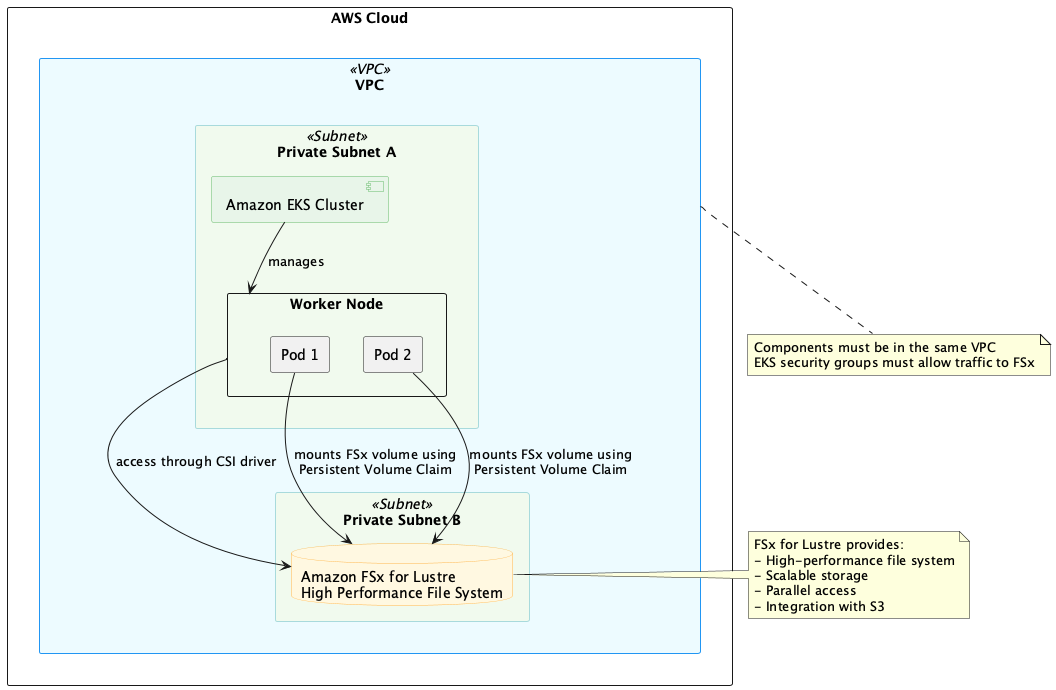
\includegraphics[width=\textwidth]{images/fsx}
    \caption{Architecture diagram showing EKS cluster connection to FSx for Lustre volume}
    \label{fig:fsx-architecture}
\end{figure}

Key features of FSx for Lustre include:
\begin{itemize}
    \item Automatic scaling of storage capacity and performance,
    \item Built--in data protection with automatic backups,
    \item Native integration with AWS services like EC2 and EKS,
    \item Support for multiple storage deployment options (scratch, persistent),
    \item Throughput capacity up to hundreds of GB per second.
\end{itemize}

The service offers two deployment types:
\begin{itemize}
    \item Scratch -- optimized for temporary storage and shorter--term processing, with higher performance,
    \item Persistent -- designed for longer--term storage with data replication and backup support.
\end{itemize}

In the context of the KubeFold project, FSx for Lustre provides high--performance storage for AlphaFold databases and computation results, as shown in Figure~\ref{fig:fsx-architecture}.
The automatic management and scaling capabilities simplify operations while maintaining the performance required for protein structure predictions.

\subsection{Amazon S3 object storage}\label{subsec:amazon-s3-object-storage}

Amazon Simple Storage Service (S3) is a cloud object storage service~\cite{aws_s3}.
It provides virtually unlimited disk space with guaranteed availability of 99.999999999\%.
It is an industry standard for cloud data storage.

The basic organizational unit in S3 are buckets.
Each bucket has a globally unique name and can store any number of objects.
Objects are identified by keys, which can contain slash characters to create a hierarchical structure.

S3 has become the standard for data storage in cloud applications.
Most modern cloud solutions provide integration with this system.
Tool providers often implement S3 support as the first choice for integrations with data stores.

The service provides a REST API interface and libraries for many programming languages.
Authentication uses digital signatures or temporary credentials.
Access control is based on IAM policies and ACL lists.
These standard mechanisms are widely used in the cloud ecosystem.

S3 provides full integration with other AWS services.
It is commonly used as storage for backups, a place to store artifacts, or the target location for computation results.
Its reliability and scalability make it the primary choice for applications requiring persistent data storage.

\subsection{AWS End User Messaging Service}\label{subsec:amazon-sns}

AWS End User Messaging is a service that enables sending SMS messages to end users~\cite{aws_messaging}.
It uses the Amazon Simple Notification Service (SNS) infrastructure to deliver messages.

The service offers the following capabilities:
\begin{itemize}
    \item sending individual SMS messages,
    \item sending group messages,
    \item monitoring delivery status,
    \item managing sending limits,
    \item automatic shortening of long messages.
\end{itemize}

The system handles two types of SMS messages:
\begin{itemize}
    \item Promotional -- optimized for cost,
    \item Transactional -- optimized for delivery reliability.
\end{itemize}

The service provides global reach through cooperation with multiple mobile operators.
Messages can be sent to over 200 countries and territories.
SNS automatically selects the best route for message delivery.

The service billing is based on the number of messages sent.
The price depends on the target country and the chosen message type.
The system offers cost control mechanisms through setting monthly spending limits.

Integration with the service is done through the REST API interface or SDK sets available for popular programming languages.
The service also provides detailed event logs and metrics available in Amazon CloudWatch.

The KubeFold platform uses AWS End User Messaging to notify researchers about the completion of protein structure calculations by the AlphaFold algorithm.
The system sends SMS messages containing information about task status and links to results in S3 storage.


\section{Cluster operator concept}

A Kubernetes operator is a program that extends cluster capabilities with automatic management of complex applications~\cite{k8s_operators}.
An operator automates tasks that would normally require manual intervention from a system administrator.

Custom Resource Definitions (CRDs) are the fundamental building blocks of an operator.
These resources define new types of objects that can be managed within a Kubernetes cluster.
The operator continuously monitors the state of these resources and performs necessary actions to keep the system running as expected.

The operator automates typical administrative tasks such as:
\begin{itemize}
    \item Installing and updating applications,
    \item Creating and restoring backups,
    \item Detecting and fixing failures,
    \item Modifying application settings.
\end{itemize}

Operators are particularly effective at managing stateful applications like databases and messaging systems.
In such cases, the operator automatically performs complex operations that typically require specialized knowledge.

An operator consists of two main parts: custom resource definitions and a management program.
The management program continuously compares the current system state with the desired state and implements necessary changes.

\subsection{Cluster operator architecture}

A Kubernetes operator follows a control loop pattern called the reconciliation loop.
This pattern continuously monitors the cluster state and makes adjustments to maintain the desired configuration.
The operator consists of several key components working together to manage custom resources.

The core components of an operator architecture include:

\begin{itemize}
    \item Custom Resource Definition (CRD) -- Defines the schema and validation rules for custom resources,
    \item Controller -- Implements the business logic and reconciliation loop,
    \item Client -- Interfaces with the Kubernetes API to read and modify resources,
    \item Cache -- Maintains an in--memory copy of watched resources for efficiency,
    \item Work Queue -- Buffers reconciliation requests to handle them sequentially.
\end{itemize}

The reconciliation loop follows these main steps:
\begin{enumerate}
    \item Watch for changes to custom resources and related Kubernetes objects,
    \item Compare current state with desired state specified in the custom resource,
    \item Calculate what changes are needed to reach desired state,
    \item Apply the necessary changes through the Kubernetes API,
    \item Update status of the custom resource.
\end{enumerate}

Figure~\ref{fig:kubernetes-operator-flow} illustrates the typical interaction flow between components in a Kubernetes operator:

\begin{figure}[htbp]
    \centering
    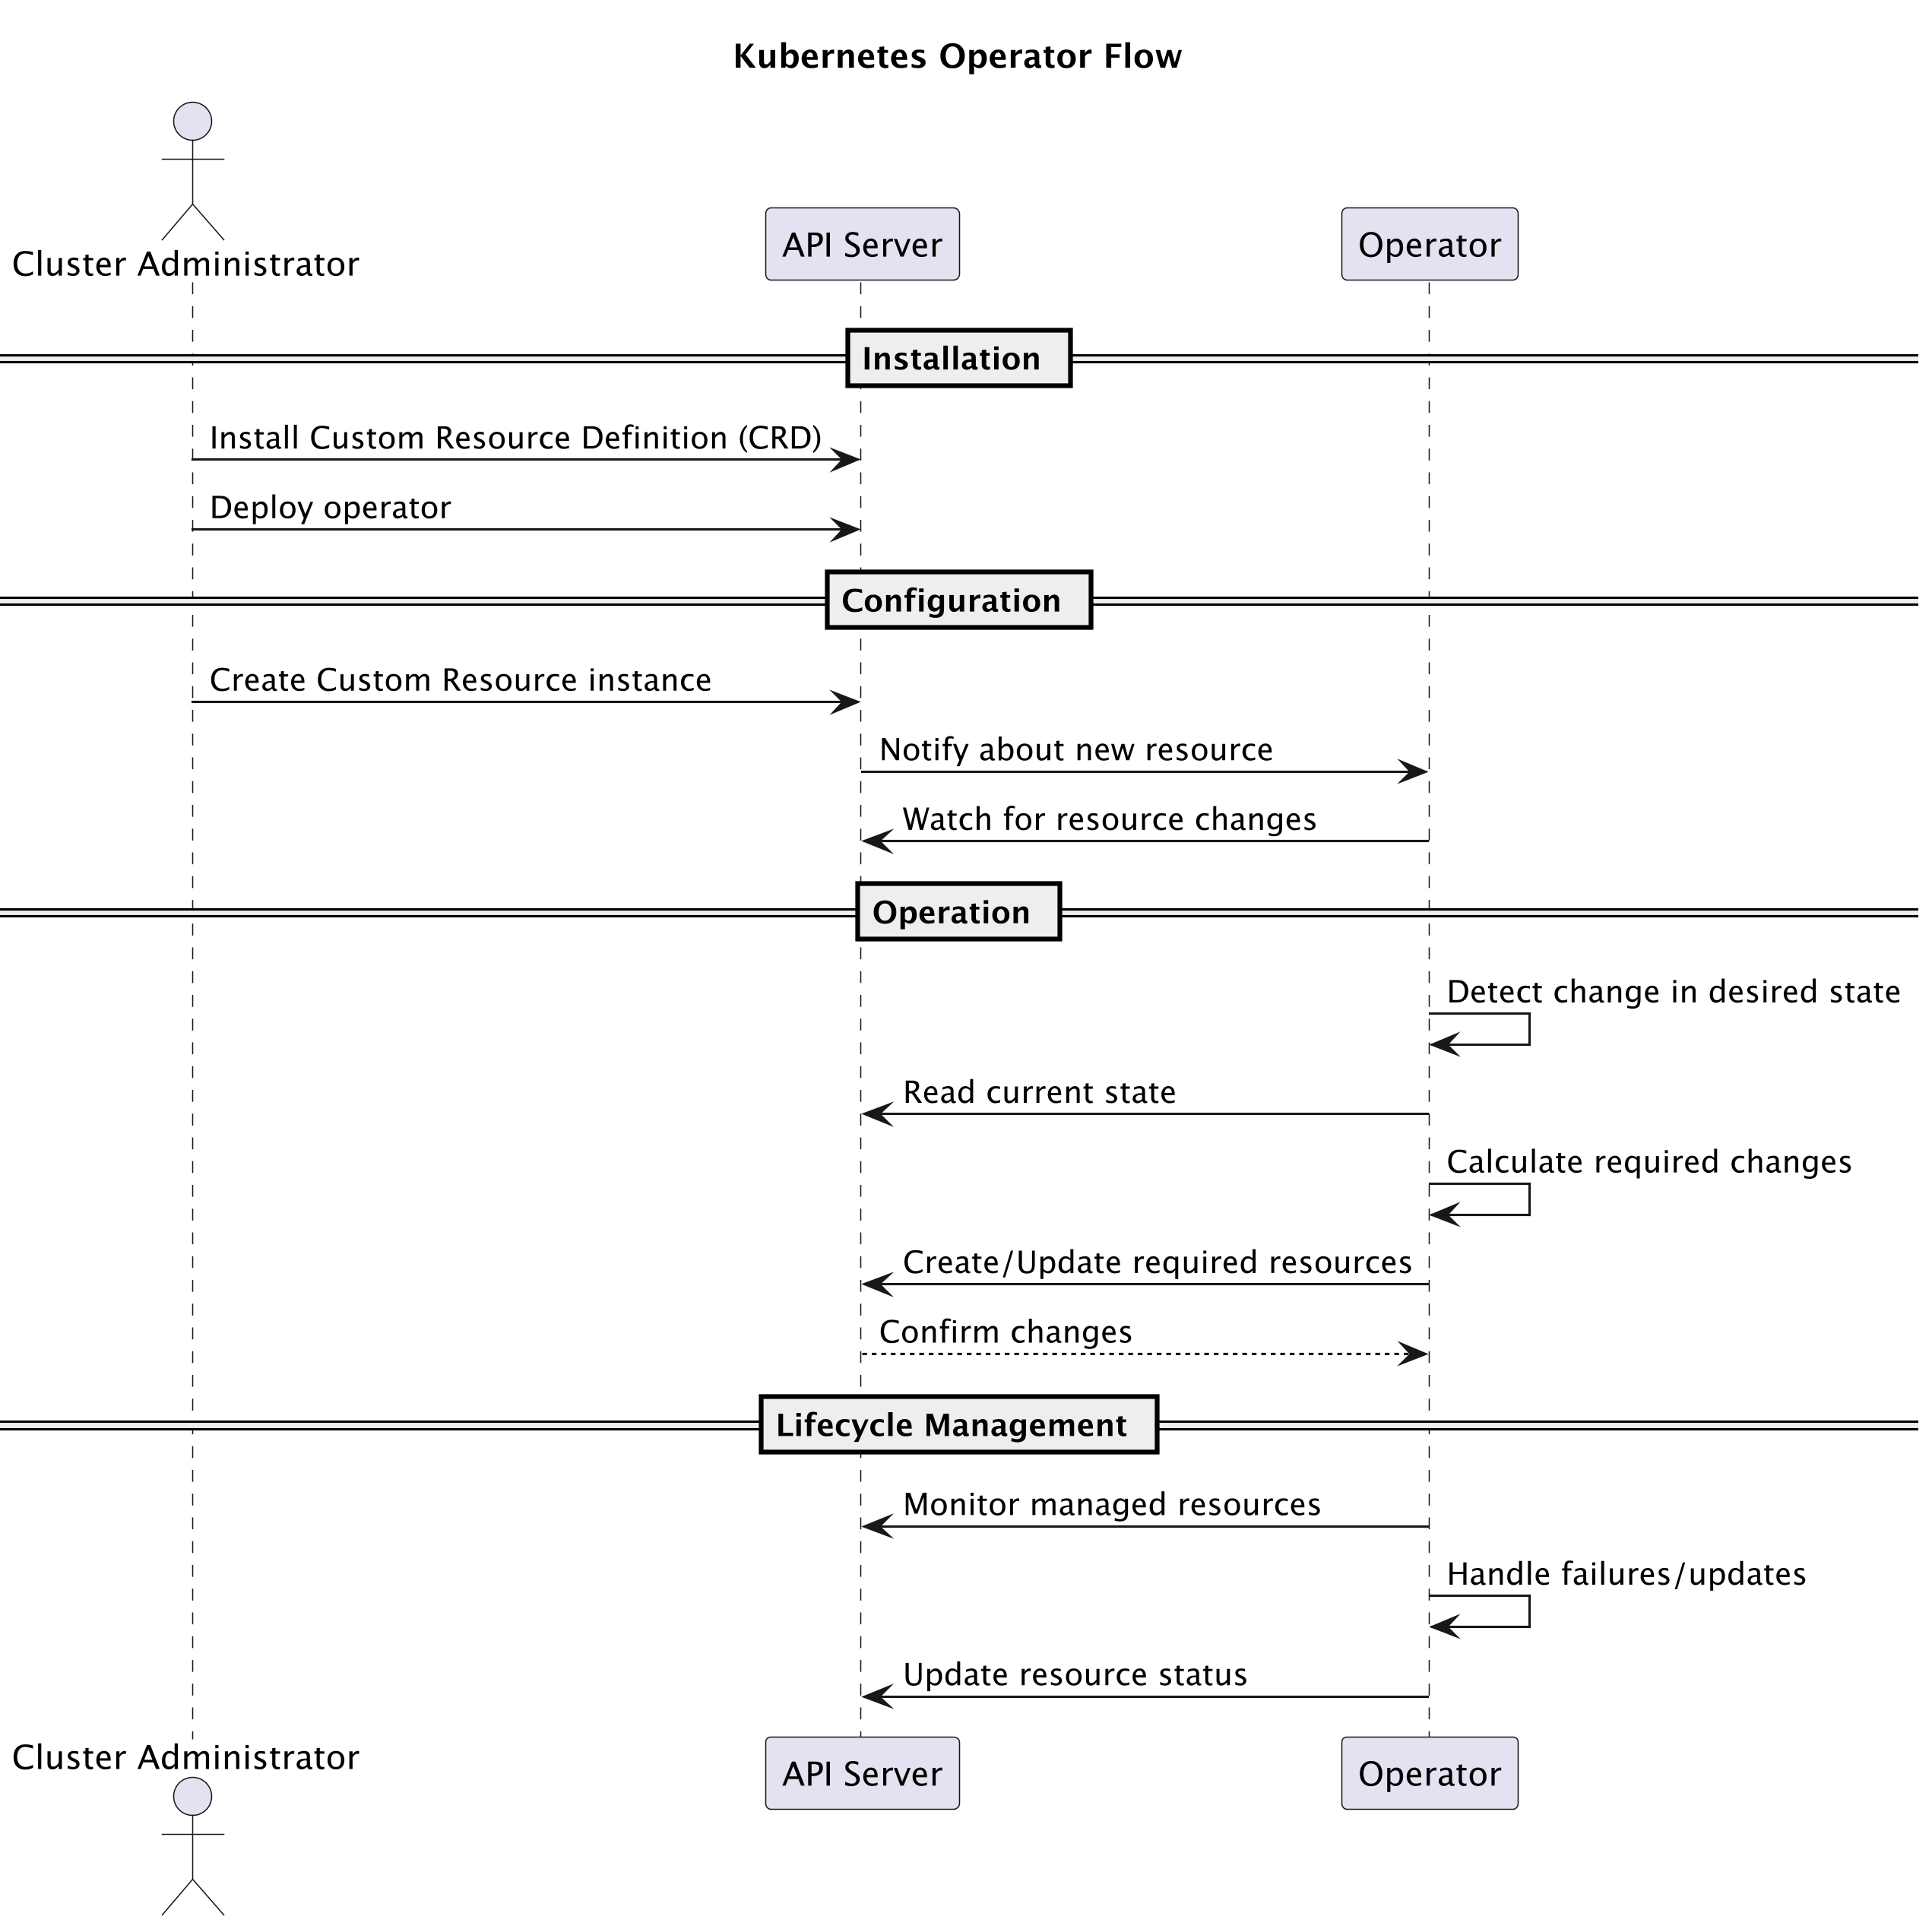
\includegraphics[width=\textwidth]{images/kubernetes_operator_flow}
    \caption{Kubernetes Operator Sequence Diagram demonstrating a reconciliation loop}
    \label{fig:kubernetes-operator-flow}
\end{figure}

The operator pattern enables domain--specific knowledge to be encoded into software that can automatically manage complex applications.
This automation reduces operational overhead and helps maintain consistency across deployments.

\subsection{Go programming language}\label{subsec:go-programming-language}

Go was created in 2007 by a Google team consisting of Robert Griesemer, Rob Pike, and Ken Thompson~\cite{golang}.
Google needed a language that would streamline the creation of large--scale server systems and simplify the software development process in large programming teams.

The first public version of the language was released in 2009.
The language was created with the intention of building scalable server systems that could handle Google's growing infrastructure.
The creators wanted to combine the simplicity of Python with the efficiency of C\@.

The main features of Go are simple syntax, built--in concurrency support, and efficient compilation.
The language offers static typing and automatic memory management.
The Go standard library provides rich support for network operations and concurrent processing.

Go introduces communication channels and goroutines as basic mechanisms for handling concurrency.
Thanks to them, creating parallel programs is much simpler than in other languages.
This is particularly useful in distributed systems.

The Go ecosystem provides tools for automatic code formatting, documentation generation, and dependency management.
Go modules enable versioning and easy code sharing.
The \texttt{go mod} tool automatically manages project dependencies.

Go is a popular choice for creating DevOps tools and cloud systems.
Kubernetes and Docker were written in Go. This language works well in projects requiring high performance and reliability.


\section{Recent Advances in Protein Structure Prediction}

\subsection{Core AlphaFold Developments}

\subsubsection{Improved protein structure prediction using potentials from deep learning (2020)}

Senior et al.
presented AlphaFold (the first version) which uses a deep neural network to predict distances between residue pairs, constructing a potential of mean force that can be optimized by gradient descent to fold the protein~\cite{Senior2020AlphaFold}.
In the CASP13 competition, this method produced high-accuracy structures for 24 out of 43 free-modeling targets, far outperforming other methods.

\subsubsection{Highly accurate protein structure prediction with AlphaFold (2021)}

Jumper et al.
introduced \textbf{AlphaFold2}, a revolution in protein structure prediction.
It regularly achieves atomic accuracy even when no homologous structure is known~\cite{Jumper2021AlphaFold2}.
Validated at CASP14, AlphaFold2's novel architecture (with an attention-based "Evoformer" and end-to-end differentiable structure module) demonstrated accuracy on par with experimental structures in a majority of cases.
This breakthrough showed that computational methods can predict protein 3D structure from sequence alone with unprecedented accuracy.

\subsubsection{Accurate structure prediction of biomolecular interactions with AlphaFold 3 (2024)}

Abramson et al.
unveiled \textbf{AlphaFold 3 (AF3)}, a substantially updated model using a \textbf{diffusion-based architecture} to predict the \textbf{joint structure of complexes} including proteins, nucleic acids, small molecules, and ions~\cite{Abramson2024AlphaFold3}.
AF3 shows markedly improved accuracy over specialized tools: it far outperforms traditional docking for protein–ligand complexes, achieves much higher accuracy on protein–DNA/RNA interactions than prior nucleic-acid-specific predictors, and greatly improves antibody–antigen complex prediction versus AlphaFold-Multimer.
This work demonstrates that a single deep-learning framework can accurately model diverse biomolecular assemblies, heralding a new era of high-accuracy multi-component complex prediction.

\subsection{Conformational Ensemble and Alternative State Prediction}

\subsubsection{Sampling alternative conformational states of transporters and receptors with AlphaFold2 (2022)}

del Alamo et al.
demonstrated that by stochastically subsampling the MSA input, AlphaFold2 can be driven to generate multiple conformations for dynamic proteins~\cite{delAlamo2022AlternativeStates}.
In tests on membrane transporters and GPCRs, this simple MSA-depth reduction yielded accurate models of distinct states (e.g. inward vs.
outward facing), with extreme conformations matching experimental structures (average TM-score ≈0.94).
This study highlighted an underexplored capability of AlphaFold2 to predict conformational ensembles and suggested the need for next-generation AI models that output biophysical state ensembles.

\subsubsection{Structure prediction of alternative protein conformations (2024)}

Bryant \& Noé developed Cfold, a neural network trained on a special "conformational split" of the PDB to predict alternative protein structures~\cite{Bryant2024Cfold}.
By ensuring that conformational variants of the same protein are separated into training vs.
test sets, Cfold can genuinely predict unseen alternative states rather than memorizing them.
The method efficiently explores a protein's conformational landscape and achieved >50\% success in predicting known alternative conformations with high accuracy (TM-score > 0.8).
Cfold demonstrates that neural networks can be adapted to generate biologically relevant conformers, addressing a gap left by AlphaFold2 which was uncertain in predicting truly novel conformations.

\subsubsection{High-throughput prediction of protein conformational distributions with subsampled AlphaFold2 (2024)}

Monteiro da Silva et al.
introduced a method to directly predict the \textbf{relative populations} of protein conformations using AlphaFold2 by subsampling MSAs~\cite{MonteiroSilva2024SubsampledAF2}.
AlphaFold2 typically predicts a single ground-state structure, but here multiple MSA subsets yield an ensemble of states.
When tested against NMR data for two proteins (Abl1 kinase and GM-CSF), the method correctly predicted changes in state populations with >80\% accuracy.
This subsampling strategy was especially effective for qualitatively predicting how mutations or evolution shift conformational landscapes, offering a fast, cost-effective way to estimate conformational distributions for applications in pharmacology and evolution.

\subsection{Physics-Informed and Dynamics-Aware Models}

\subsubsection{Protein Conformation Generation via Force-Guided SE(3) Diffusion Models (2024)}

Wang et al.
introduced ConfDiff, a deep generative model that integrates physical knowledge (forces) into the SE(3)-equivariant diffusion process for protein structure generation~\cite{Wang2024ConfDiff}.
Traditional diffusion models sample protein conformations but can deviate from true equilibrium distributions due to lack of physics.
ConfDiff addresses this by coupling a learned force field with score-based diffusion: the force-guided network steers sampling toward realistic basins, yielding diverse conformations that maintain high fidelity to the native ensemble.
In experiments on 12 fast-folding proteins and BPTI, ConfDiff surpassed prior state-of-the-art methods in capturing native conformational variability. \textit{(Presented at ICML 2024)}

\subsubsection{Simultaneous Modeling of Protein Conformation and Dynamics via Autoregression (2025)}

Shen et al.
proposed \textbf{ConfRover}, the first model to learn \textbf{protein conformational dynamics and structures simultaneously} from MD trajectories~\cite{Shen2025ConfRover}.
ConfRover uses a modular autoregressive design: (i) an encoder adapted from folding models that embeds each time-frame conformation, (ii) a sequence model that captures temporal dependencies between frames, and (iii) an SE(3) diffusion decoder that generates 3D structures for each step.
This enables both time-dependent (trajectory) generation and time-independent sampling of conformations within one framework.
On the large ATLAS MD dataset, ConfRover successfully learned complex motions and could generate realistic trajectories, marking a significant step toward integrating \textit{dynamic behavior} into structure prediction. \textit{(Preprint, May 2025)}

\subsection{Novel Architectural Approaches}

\subsubsection{Structure Language Models for Protein Conformation Generation (2024)}

Lu et al.
proposed a novel framework called \textbf{Structure Language Modeling (SLM)} for efficient generative modeling of protein conformations~\cite{Lu2024SLM}.
Instead of operating purely in 3D coordinate space, SLM first encodes protein structures into a compact latent representation via a discrete VAE, then applies \textbf{conditional language models} to capture sequence-conditioned conformation distributions.
This approach enabled \textbf{20–100× faster} generation of diverse conformations compared to 3D diffusion methods, by exploring ensemble modes in a more tractable latent space.
The authors instantiated SLM with transformer architectures (including a BERT-like model fine-tuned from ESM) and demonstrated its ability to model equilibrium dynamics (e.g. BPTI), conformational changes, and even disordered protein ensembles with high efficiency. \textit{(ICLR 2025 conference paper)}

\subsection{Comprehensive Reviews and Surveys}

\subsubsection{Protein structure prediction via deep learning: an in-depth review (2025)}

Meng et al.
provided a comprehensive review of deep learning techniques for protein structure prediction~\cite{Meng2025DeepLearningReview}.
This article surveys how various architectures – from CNNs and RNNs to GNNs and large language models (LLMs) – have been applied to protein folding.
It discusses advances in databases and resources, evaluates state-of-the-art methods (e.g. AlphaFold2, RoseTTAFold, ESMFold) and their impact on drug discovery, and highlights future challenges.
Key issues identified include the need for improved interpretability of deep models, handling multi-domain and flexible regions, and incorporating dynamics and multi-molecule interactions into predictions.
The review concludes that despite recent breakthroughs, there remains ample room for improving prediction of protein dynamics, complex assemblies, and functional annotations.


\section{Automation of Bioinformatics Workflows}

The scientific literature proposes a range of patterns and tools for managing the infrastructure required for machine learning computations, with particular emphasis on cloud-based solutions and container orchestration.
To understand the current landscape, it is essential to examine both traditional workflow orchestration tools and specific deployment approaches that have emerged in recent years.

\subsection{Traditional Workflow Orchestration Tools}

While specialized bioinformatics platforms provide powerful capabilities, it is important to examine the broader landscape of workflow orchestration tools that have become standard in the field.
These tools, while effective for workflow definition and execution, reveal critical limitations when it comes to infrastructure management -- a gap that operator-based solutions like KubeFold are designed to address.

The bioinformatics community has adopted several workflow management systems, each with distinct characteristics and approaches~\cite{workflows_review_nature}.

\textbf{Nextflow} is a dataflow-based workflow manager that has gained significant popularity in the bioinformatics community.
It provides excellent documentation, supports both Conda environments and container technologies, and offers good integration with cloud platforms.
Nextflow uses a dataflow programming model where processes are connected via their outputs and inputs, enabling automatic parallelization~\cite{nextflow}.
The nf-core community has created a substantial collection of peer-reviewed bioinformatics pipelines, demonstrating the tool's adoption and utility.

\textbf{Snakemake} follows a Make-like approach where users specify output files they want to build, and the system determines the necessary steps to create them.
It is Python-based, making it accessible to researchers familiar with Python, and provides strong support for reproducibility through built-in environment management~\cite{snakemake}.
Snakemake offers excellent support for incremental builds and re-entrancy, allowing workflows to resume from interruption points.

\textbf{Galaxy} provides a web-based platform that abstracts workflow complexity behind a graphical user interface.
It enables researchers without programming expertise to construct and execute complex bioinformatics workflows~\cite{galaxy}.
Galaxy's strength lies in its accessibility and the extensive tool ecosystem, with thousands of pre-configured bioinformatics tools available through its interface.

\textbf{Workflow Description Language (WDL)} and its execution engine \textbf{Cromwell} offer a declarative approach to workflow specification.
WDL provides a standardized way to describe workflows that can be executed across different environments, promoting portability~\cite{wdl_cromwell}.
The approach separates workflow logic from execution details, enabling the same workflow to run on various computing platforms.

\textbf{Common Workflow Language (CWL)} represents an effort to standardize workflow descriptions across different execution engines.
CWL workflows can be executed by multiple workflow runners, providing workflow portability across different computational environments~\cite{cwl}.

Despite their sophistication in workflow orchestration, these traditional tools exhibit significant limitations regarding infrastructure management that highlight the value of operator-based approaches:

\textbf{Manual Infrastructure Provisioning}: All of these workflow systems require pre-existing computational infrastructure.
Users must manually provision clusters, configure networking, set up storage systems, and manage resource allocation before executing workflows.
This places a substantial operational burden on researchers and requires specialized DevOps knowledge.

\textbf{Limited Cloud-Native Integration}: While these tools can execute on cloud platforms, they do not leverage cloud-native technologies like Kubernetes operators for automated infrastructure management.
They treat cloud resources as static infrastructure rather than dynamically managed, declarative resources.

\textbf{Lack of Automated Scaling}: Traditional workflow managers provide limited support for automatic infrastructure scaling in response to workload demands.
Resource allocation is typically configured at deployment time rather than adjusted dynamically based on queue depth or resource utilization.

\textbf{Complex Deployment Requirements}: Deploying these workflow systems in production environments requires significant configuration effort.
Setting up proper cluster managers, configuring security policies, implementing backup strategies, and ensuring high availability demands extensive operational expertise.

\textbf{Separation of Concerns}: These tools excel at workflow orchestration but delegate infrastructure concerns to external systems.
This separation, while following good architectural principles, results in complex operational overhead when researchers need to manage both workflow logic and underlying infrastructure.

\subsection{Foldy}

In the paper \textit{Foldy: a web application for interactive protein structure analysis}, the authors propose a complete deployment of the \textit{Foldy} application on a Kubernetes cluster, using Helm for automated installation and configuration~\cite{foldy,helm}.
The application allows users without advanced bioinformatics knowledge to predict protein structures (AlphaFold), dock ligands (DiffDock, AutoDock Vina), and visualize domains (Pfam).

The application deployment process assumes:
\begin{itemize}
    \item manual provisioning of infrastructure resources: domain name, static IP address, Kubernetes cluster, and database;
    \item automatic deployment of the frontend, backend, and computational workers with a single \texttt{helm install} command;
    \item the ability to run workers locally (on private resources) using a Docker image or bash scripts if Docker is not supported.
\end{itemize}

Foldy uses a task queue mechanism (RedisQueue), and computational workers are scaled dynamically using KEDA and Prometheus.
This approach allows prediction of large protein structures (up to 3000 amino acids) and supports thousands of users~\cite{foldy}.

Table~\ref{tab:foldy-kubefold-comparison} presents a comparison between Foldy and KubeFold across key operational dimensions:

\begin{table}[htbp]
\centering
\caption{Comparison of Foldy and KubeFold platforms}
\label{tab:foldy-kubefold-comparison}
\begin{tabular}{|l|p{5.5cm}|p{5.5cm}|}
\hline
\textbf{Aspect} & \textbf{Foldy} & \textbf{KubeFold} \\
\hline
\textbf{Installation} & 
Requires manual infrastructure provisioning (DNS, cluster, databases), then single \texttt{helm install} command & 
Complex initial setup with Kubernetes operator deployment, but automated resources management afterwards \\
\hline
\textbf{User Interface} & 
Web--based graphical interface & 
YAML configuration files providing declarative infrastructure management \\
\hline
\textbf{Scale} & 
Supports hundreds of users with correctly configured scaling via KEDA & 
Designed for large organizations--automatic resource management and cloud--native scaling \\
\hline
\textbf{Automation Level} & 
Automated workflow execution and scaling, manual infrastructure setup & 
Complete lifecycle automation including job management, artifacts archiving, notifications and cleanup \\
\hline
\textbf{DevOps Requirements} & 
Moderate -- requires initial cluster setup, DNS configuration, and database management & 
High initial setup complexity, minimal ongoing operational overhead due to operator--based automation \\
\hline
\textbf{Target Audience} & 
Researchers and biologists without programming expertise & 
Technical teams and institutions requiring enterprise--grade automation and cloud-native solution \\
\hline
\end{tabular}
\end{table}

\textbf{Limitation:} While Foldy provides a powerful and user-friendly platform, its deployment still requires significant manual configuration and integration effort.
Deployment still involves some infrastructure setup, including configuring DNS, cluster resources, and databases, which can be complex for teams without DevOps experience.
Additionally, monitoring and logging are not provided out-of-the-box and require further setup.
Although some operational tasks can be partially automated, there is no centralized layer managing the full lifecycle of jobs, storage, and infrastructure after deployment.

\subsection{A Comprehensive Cloud Architecture for Machine Learning-enabled Research}

In the paper \textit{A Comprehensive Cloud Architecture for Machine Learning-enabled Research}~\cite{cloud_architecture_for_research}, the authors present a comprehensive architecture deployed at the Texas Advanced Computing Center.
The proposed infrastructure includes:
\begin{itemize}
    \item virtualization using OpenStack (with GPU support via PCI passthrough);
    \item container orchestration using Kubernetes (deployed via Kubespray);
    \item access to GPU-enabled JupyterHub as an interactive interface for researchers;
    \item ability to run long-term services (e.g., inference) via the Tapis Pods API;
    \item orchestration of complex workflows via Tapis Workflows.
\end{itemize}

The architecture enables the execution of machine learning models, data management, and training of models on HPC clusters via an HTTP interface.
Thanks to integration with the Tapis ML Hub, users can search for, deploy, and use pre-trained models from Hugging Face without the need to build them from scratch.

\textbf{Limitation:} Although highly capable, the proposed architecture requires coordination across multiple layers of the stack -- OpenStack, Kubernetes, Tapis services -- which demands specialized knowledge and operational overhead.
GPU provisioning, workflow orchestration, and model deployment are fragmented across various APIs and services, making end-to-end automation challenging for small teams or institutions without dedicated infrastructure engineers.
While powerful in production settings, the architecture lacks a unified interface for researchers to independently manage job submissions, monitoring, and data without DevOps support.

Moreover, Tapis offers an imperative approach to infrastructure management. In contrast, KubeFold offers a declarative approach to infrastructure management, and therefore the user does not need to worry about how to manage infrastructure, only defines the desired state of the system. The KubeFold operator makes decisions on how to achieve that state.

\subsection{The Value of Operator-Based Approaches}

The limitations of traditional workflow orchestration tools demonstrate the value proposition of operator-based solutions like KubeFold.
By integrating workflow management with infrastructure automation through Kubernetes operators, KubeFold addresses the operational gap that exists between workflow definition and infrastructure management.

Where existing solutions require DevOps expertise for proper deployment, KubeFold abstracts infrastructure complexity behind declarative resource definitions.
Where conventional workflow managers treat infrastructure as static, KubeFold provides dynamic resource management that adapts to computational demands.

This integration represents a fundamental shift from treating infrastructure as a prerequisite to treating it as an automatically managed component of the scientific computing platform.

\section{Summary and Identified Gaps}

Both Foldy and the described cloud architecture confirm the growing importance of Kubernetes and cloud-native tools in bioinformatics research.
Kubefold, on the other hand, offers a new quality -- shifting the burden of deployment and configuration from the user to the system, thus democratizing access to advanced AI tools in science.

The key difference between these solutions lies in their level of automation and abstraction: while Foldy provides a ready-to-use web application requiring manual infrastructure setup, and the comprehensive cloud architecture offers powerful but complex multi-layered services, Kubefold focuses on complete automation of the entire lifecycle -- from infrastructure provisioning to job monitoring -- enabling researchers to focus on scientific work rather than operational tasks.

By "Complete automation of the entire lifecycle" we mean managing aspects such as:
\begin{itemize}
  \item downloading databases
  \item deleting databases when they are no longer needed
  \item managing dependencies between different resources in the system (protein conformation prediction job and downloaded database)
  \item notifying users about computation status
  \item archiving artifacts
  \item error handling
\end{itemize} 

The review of existing solutions reveals a significant gap: while powerful cloud architectures and specialized bioinformatics platforms exist, there is a lack of solutions that seamlessly integrate automation, AI algorithms, Kubernetes orchestration, and cloud-native approaches into a unified platform.
This gap represents the primary motivation for developing KubeFold as a comprehensive solution for automated protein structure prediction in cloud environments.

    %! suppress = MissingLabel


\chapter{System design and implementation}
This chapter discusses the architecture and implementation of the KubeFold project.


\section{KubeFold platform concept}
KubeFold is software that operates on the Kubernetes platform in Operator manner.
The project consists of the following components:
\begin{itemize}
    \item Kubernetes Operator -- a component that manages business logic.
    It ensures proper deployment and management of pods responsible for downloading protein databases and performing computations.
    This component is described in detail in section~\ref{subsec:component-operator}.
    \item Downloader Component -- controls the process of downloading and decompressing protein databases.
    A detailed description can be found in section~\ref{subsec:component-downloader}.
    \item Manager Component -- handles additional operations around computations such as artifact delivery or sending notifications.
    It is described in section~\ref{subsec:component-manager}.
\end{itemize}

Additionally, KubeFold introduces two Custom Resource Definitions (CRDs).
The first is the \texttt{ProteinDatabase} resource.
It represents a single installation of a protein database in the cluster.
An example resource code is shown in listing~\ref{lst:protein_database}.
In the resource specification, users can select which databases should be installed.
Furthermore, they can specify which StorageClass should be used for the volume storing the data.
This enables specifying a class that corresponds to the Lustre file system (described in section~\ref{subsec:lustre-volumes}).
In the example code, the class named \texttt{fsx-sc} is specified, which connects to AWS FSx for Lustre volumes (see~\ref{subsec:amazon-fsx-for-lustre}).
From the user's perspective, this resource can be managed using \texttt{kubectl} as shown in figure~\ref{fig:proteindatabase_terminal}.

\begin{lstlisting}[language=yaml,caption={Example \texttt{ProteinDatabase} resource definition},label={lst:protein_database}]
#file: noinspection KubernetesUnknownResourcesInspection
apiVersion: data.kubefold.io/v1
kind: ProteinDatabase
metadata:
  name: proteindatabase-sample
spec:
  datasets:
    bfd: true
    mgyclusters: true
    nt: true
    pdb: true
    pdbseqreq: true
    rfam: true
    rnacentral: true
    uniref90: true
    uniprot: true
  volume:
    storageClassName: fsx-sc
\end{lstlisting}

\begin{figure}[htbp]
    \centering
    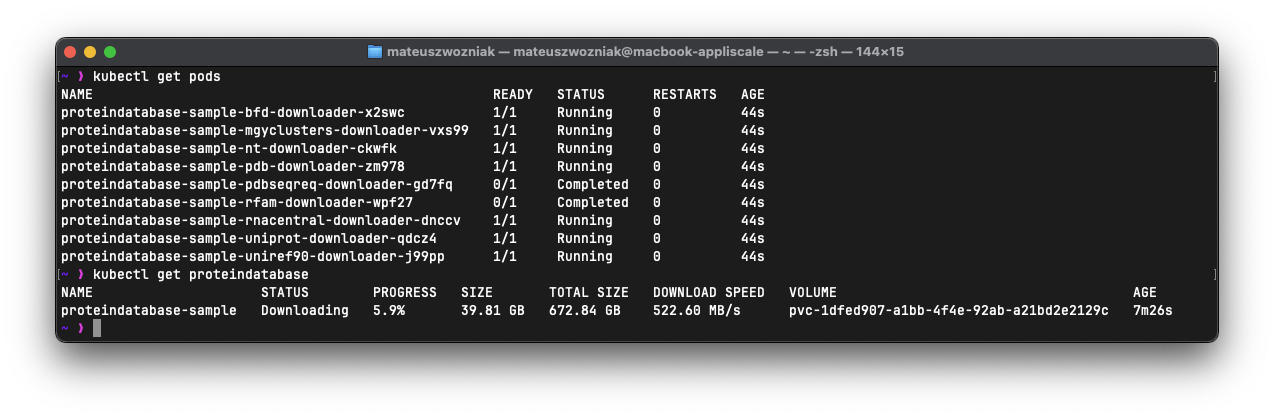
\includegraphics[width=\textwidth]{images/old_proteindatabase_terminal}
    \caption{Terminal output presenting \texttt{ProteinDatabase} resource}
    \label{fig:proteindatabase_terminal}
\end{figure}

Additionally, KubeFold supports the \texttt{ProteinConformationPrediction} resource definition.
It represents a single protein conformation computation based on a provided amino acid sequence.
An example definition is shown in listing~\ref{lst:protein_conformation_prediction}.
Users can specify task settings such as:
\begin{itemize}
    \item the protein database that the AlphaFold algorithm should use for searching,
    \item the amino acid sequence as a string of letters,
    \item settings for the volume storing temporary computation files,
    \item specification of the AlphaFold model weights source.
    In the example code, the source is set as a remote HTTP server.
    \item target location for artifacts.
    In the current version of KubeFold, only AWS S3 object storage is supported (see~\ref{subsec:amazon-s3-object-storage}).
    \item notification options.
    The example code has a single SMS notification configured for a phone number.
\end{itemize}
Management can be done using \texttt{kubectl} as shown in figure~\ref{fig:proteinconformationprediction_terminal}.

\begin{figure}[htbp]
    \centering
    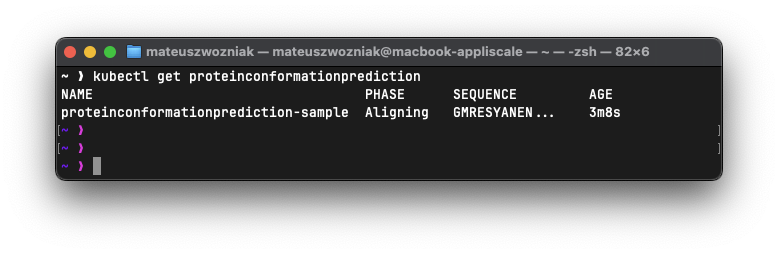
\includegraphics[width=\textwidth]{images/old_proteinconformationprediction_terminal}
    \caption{Terminal output presenting \texttt{ProteinConformationPrediction} resource}
    \label{fig:proteinconformationprediction_terminal}
\end{figure}

\begin{lstlisting}[language=yaml,caption={Example \texttt{ProteinConformationPrediction} resource definition},label={lst:protein_conformation_prediction}]
#file: noinspection KubernetesUnknownResourcesInspection
apiVersion: data.kubefold.io/v1
kind: ProteinConformationPrediction
metadata:
  name: proteinconformationprediction-sample
spec:
  database: proteindatabase-sample
  protein:
    id: [ 'A','B' ]
    sequence: GMRESY...LQQANDLKQG
  model:
    volume:
      storageClassName: fsx-sc
    weights:
      http: https://staticfilehosting.com/af3.bin.zst
    seeds:
      - 1
  destination:
    s3:
      bucket: kubefold-artifacts-sample
      region: eu-central-1
  notify:
    region: eu-central-1
    sms:
      - "+48140690323"
\end{lstlisting}


\section{Technology stack}
All three components were written in Go version 1.24 (more about it in a section~\ref{subsec:go-programming-language}).
This was a natural choice, as Go is the de facto standard for cloud software development.
The source code of the components was archived in the Git repository~\cite{git} on GitHub\cite{github}.

To compile the application and package executable files into a container image, the standard Docker builder was used.

Container images were distributed via the GitHub Container Registry (\textit{ghcr.io})~\cite{ghcr}.
Images were automatically built upon every push tag to Git by the GitHub Actions tool~\cite{github_actions}.
The workflow is shown in figure~\ref{fig:docker-images-flow}.

\begin{figure}[htbp]
    \centering
    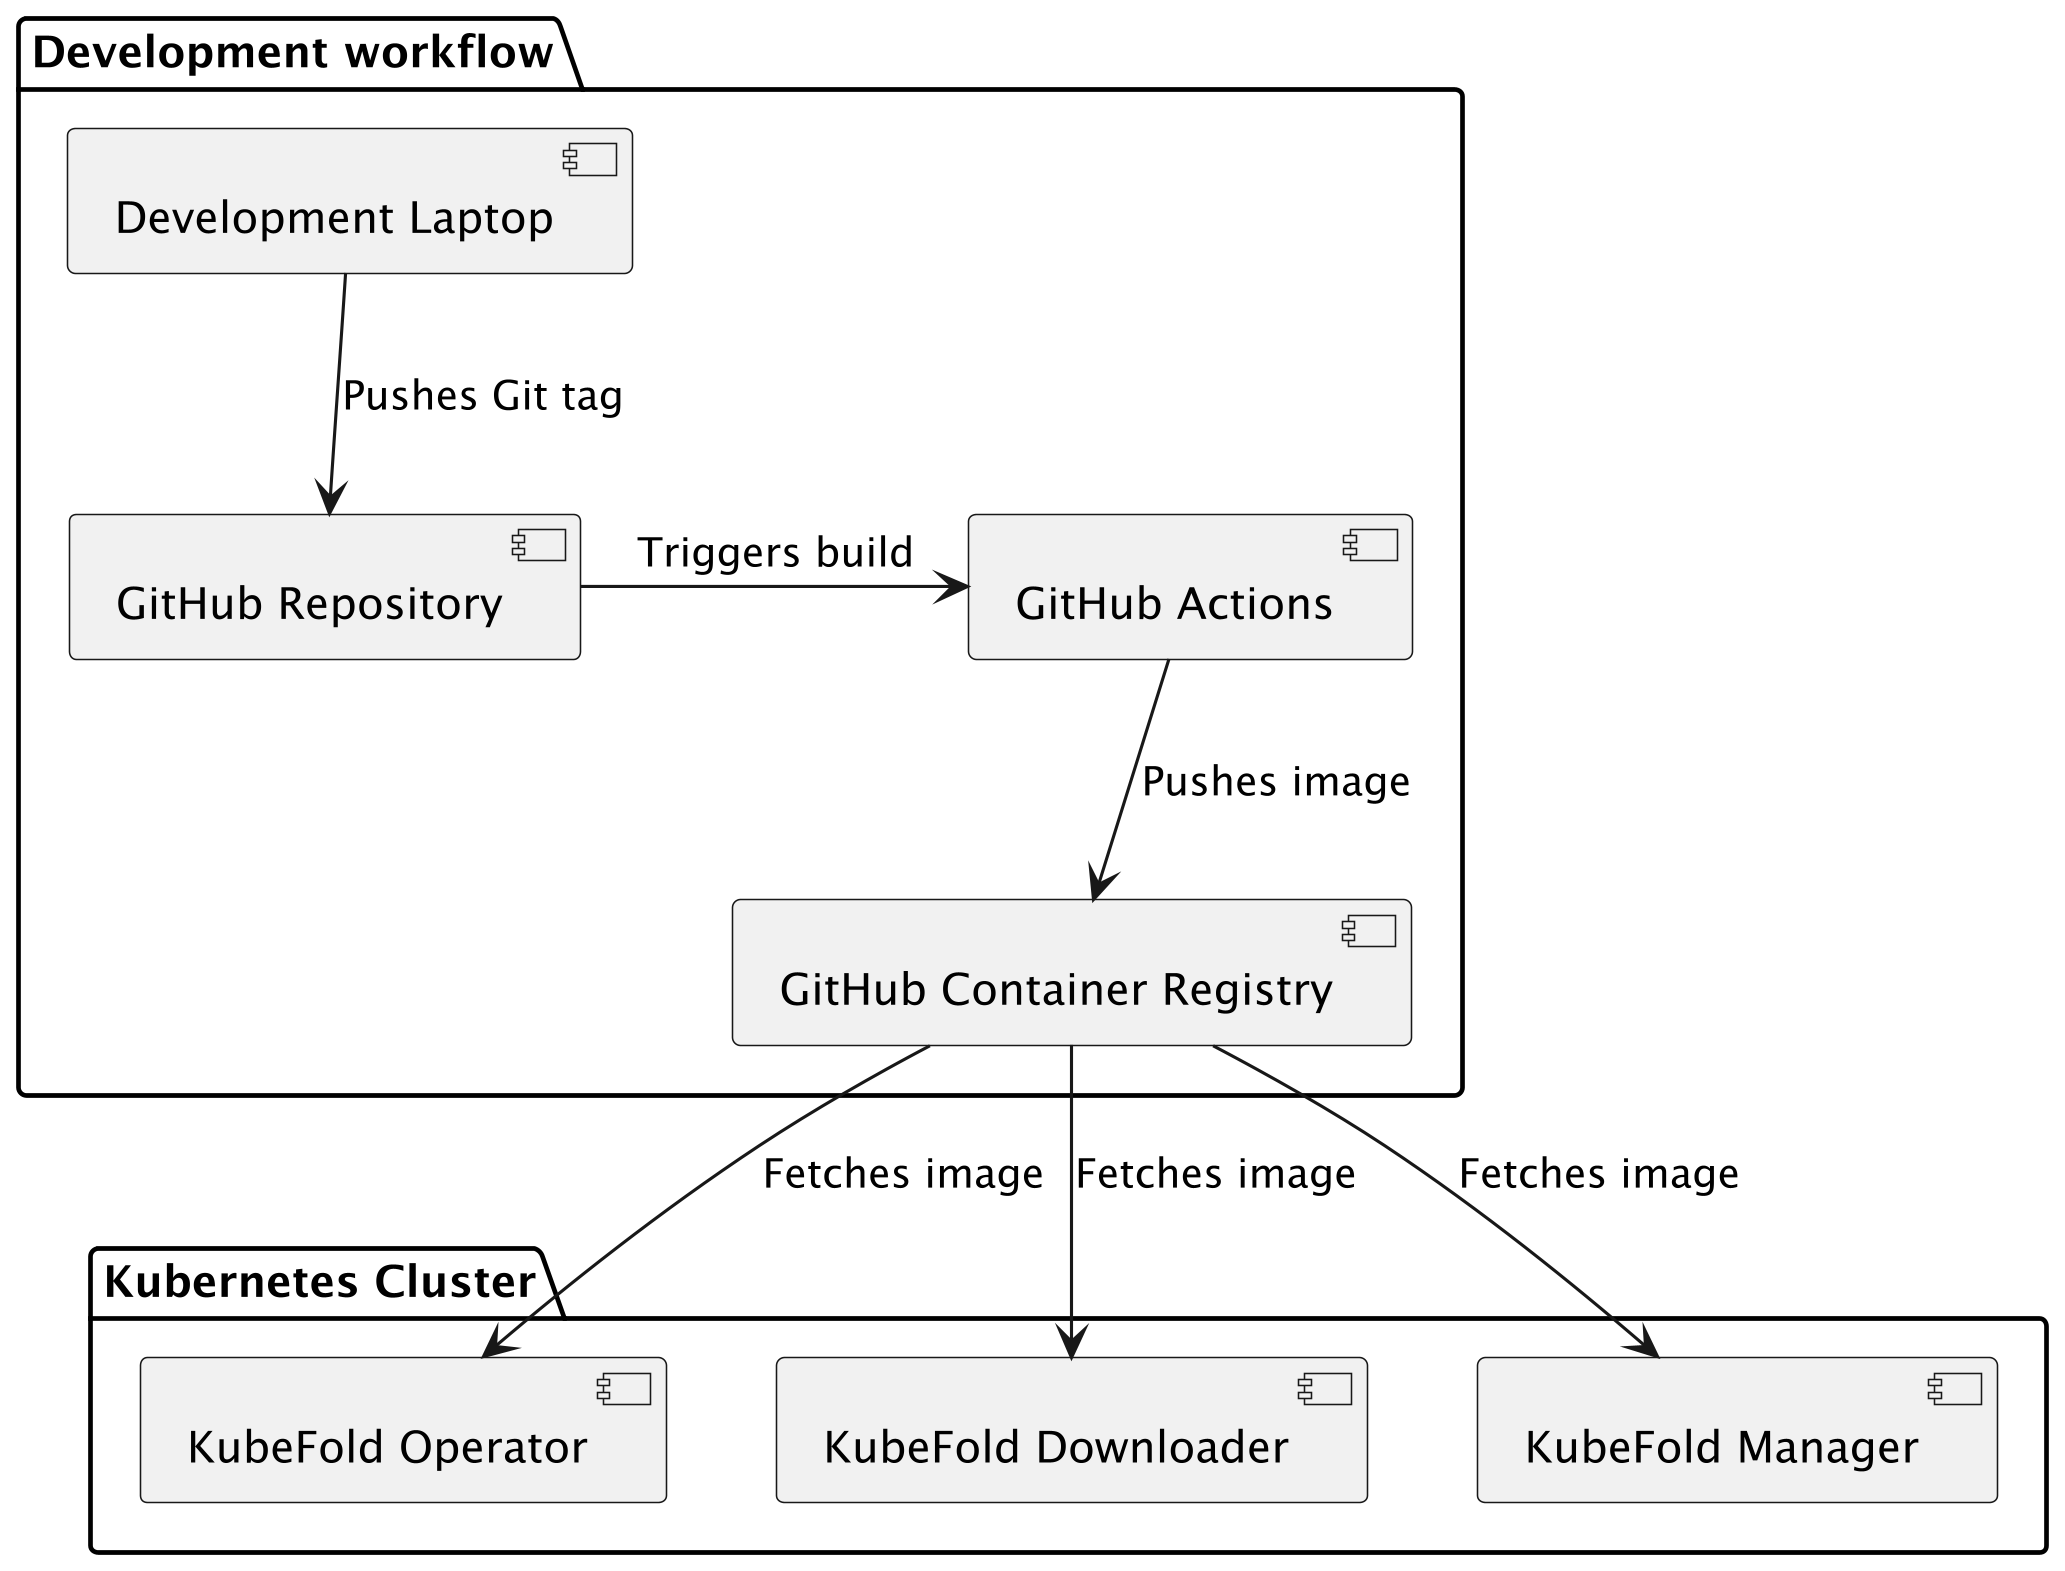
\includegraphics[width=0.8\textwidth]{images/images}
    \caption{Development workflow between GitHub and cluster}
    \label{fig:docker-images-flow}
\end{figure}

The Kubernetes Operator component (described in more detail in~\ref{subsec:component-operator}) was created based on the KubeBuilder framework~\cite{kubebuilder}.
KubeBuilder is a framework that facilitates writing native Kubernetes operators.
It creates project directory structure and immediately provides management of elements such as:
\begin{itemize}
    \item Leader election -- some operator instances can run on multiple cluster nodes simultaneously, but if there is a need to select a single distinguished instance, the leader election selects it,
    \item Generation of installation scripts -- KubeBuilder has the ability to generate ready--to--use installation scripts that can later be used for automatic operator installation and all its dependencies in the cluster with a single \texttt{kubectl apply} command,
    \item Role and permission definitions.
    Kubernetes uses an authorization model called \textit{RBAC} (Role--Based Access Control)~\cite{k8s_rbac}.
    KubeBuilder checks what permissions an operator instance should have and ensures that the appropriate permissions are granted to it.
\end{itemize}


\section{System architecture}

Both introduced CRD resources manage certain subordinate resources.

The \texttt{ProteinDatabase} resource primarily creates: a persistent volume claim that will store data from protein databases and a set of jobs that correspond to downloading individual databases.
The resource dependency architecture is shown in figure~\ref{fig:proteindatabase}.
The number of jobs is exactly the same as the number of selected databases defined in the YAML code.
Due to this split process of downloading, it is possible for multiple nodes to download independent data at the same time.
In such a case, the total throughput increases, as it will not be limited by the speed of the single node network interface.
All pods created by the jobs connect to a common volume and download databases from Google servers using HTTP protocol.
The progress is logged to the \texttt{stdout} of the container in real time.
This enables the operator to read container logs and monitor progress in real time.
Pods and volume are connected to the \texttt{ProteinDatabase} resource using the \textit{ownerReferences} mechanism.
If the parent resource is deleted, the subordinate resources will also be automatically deleted.
The automatic resource cleanup functionality is handled in the Kubernetes implementation, not in the operator.

\begin{figure}[htbp]
    \centering
    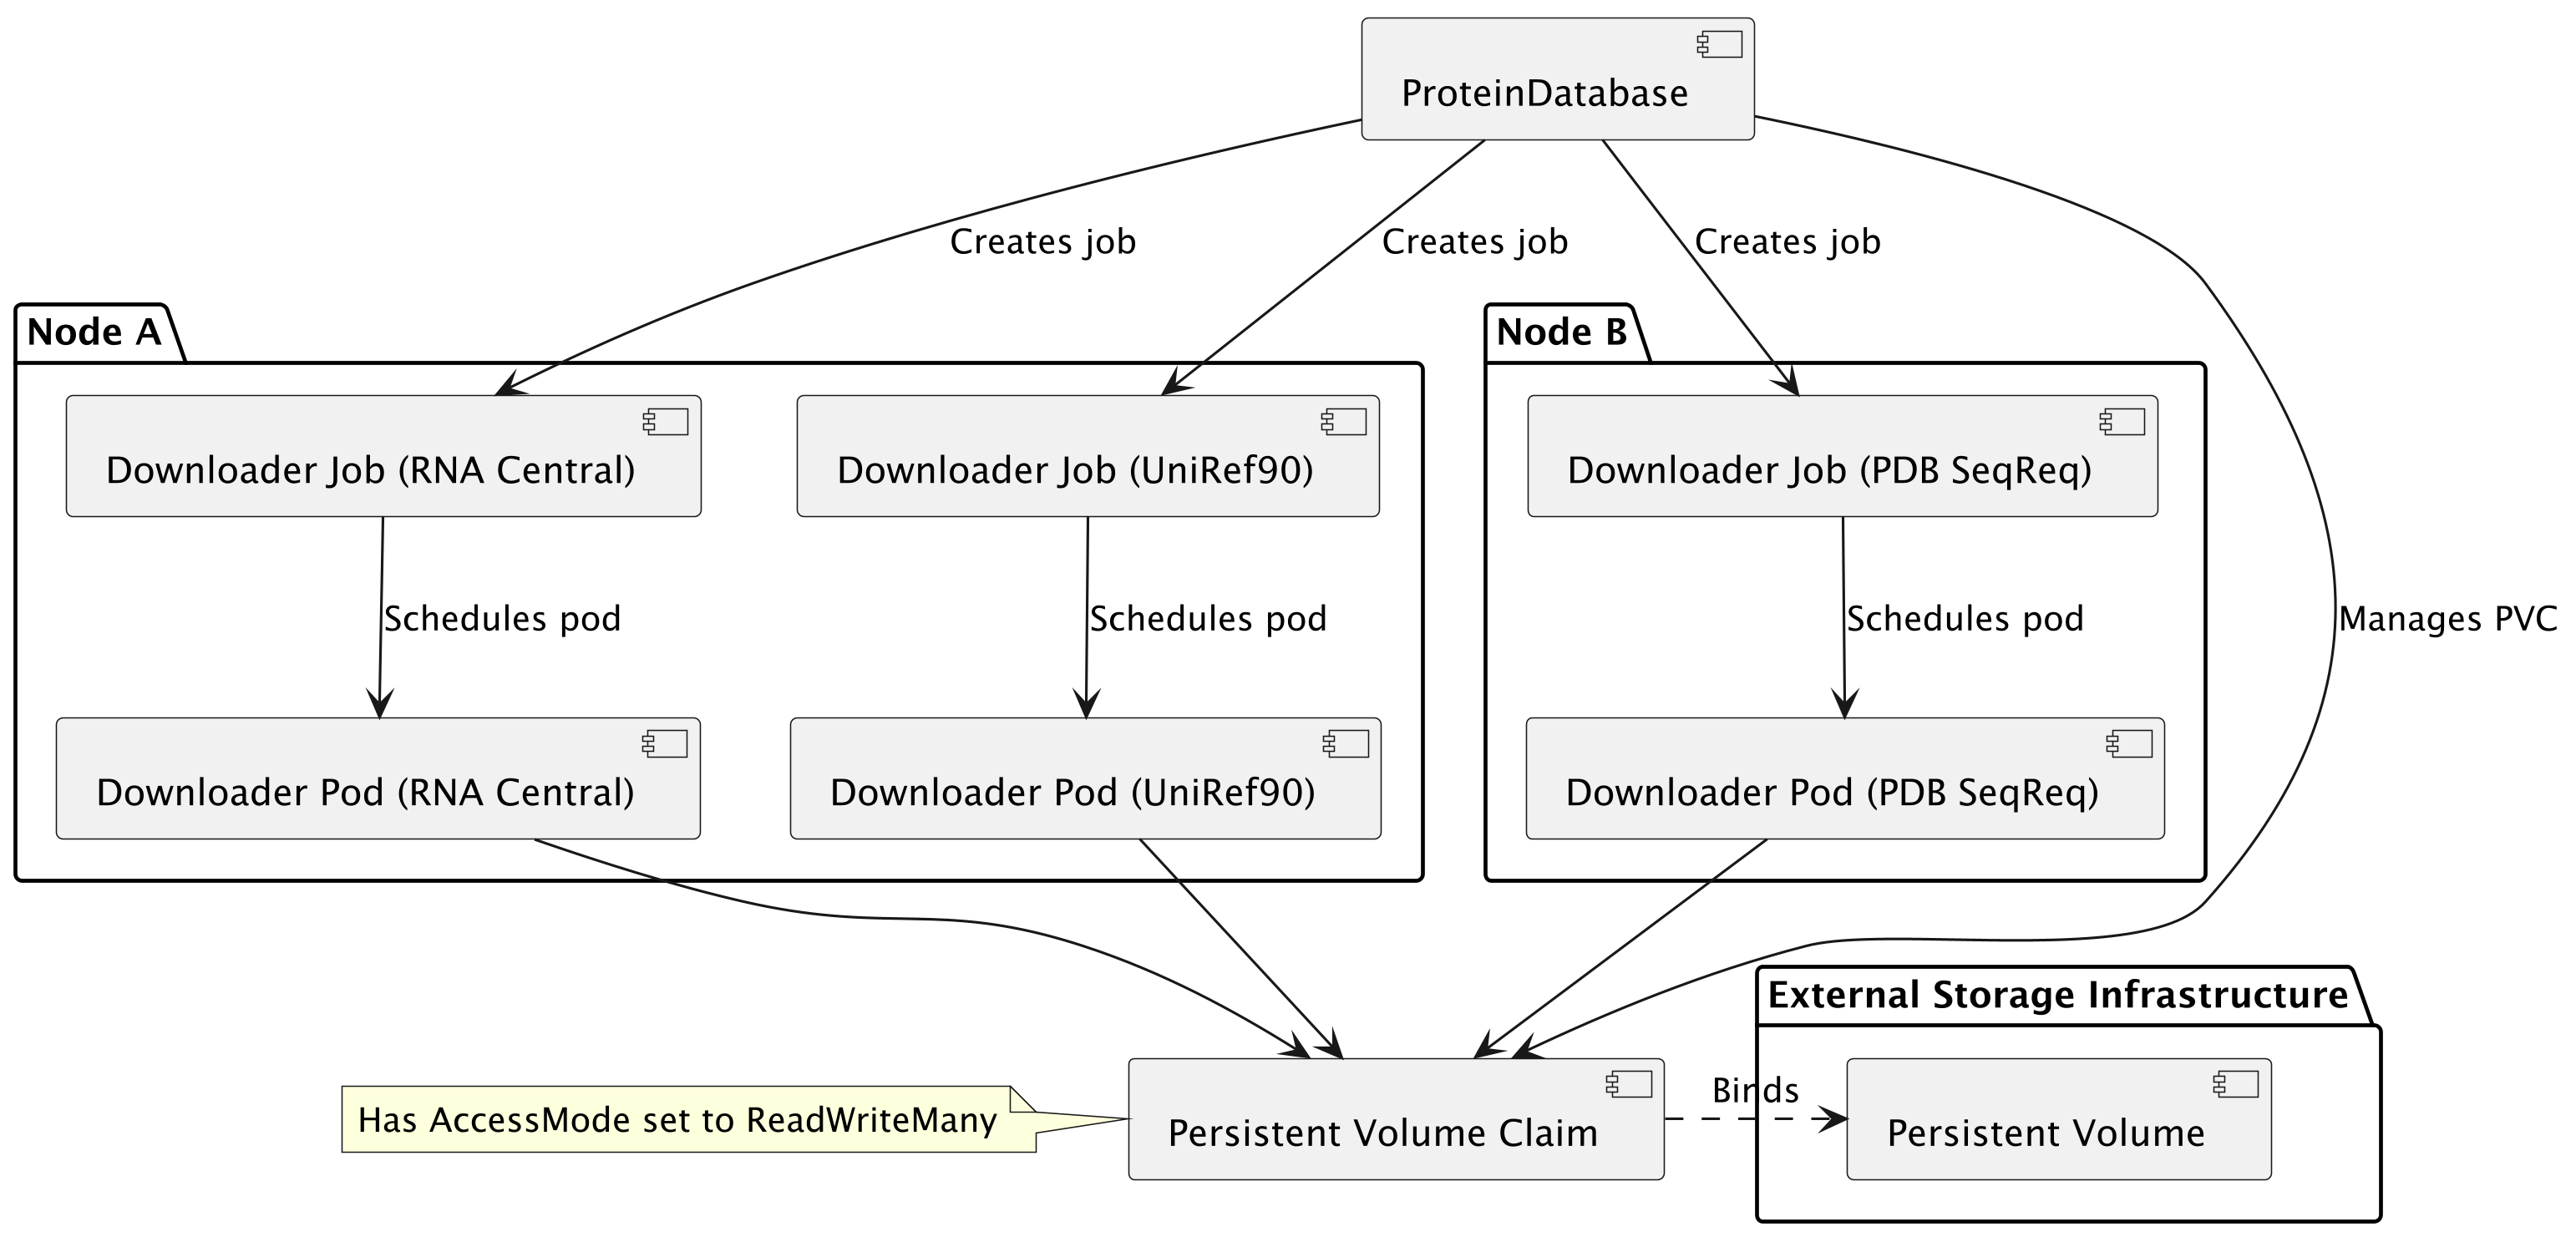
\includegraphics[width=\textwidth]{images/proteindatabase}
    \caption{Cluster resource architecture of ProteinDatabase}
    \label{fig:proteindatabase}
\end{figure}

\begin{figure}[htbp]
    \centering
    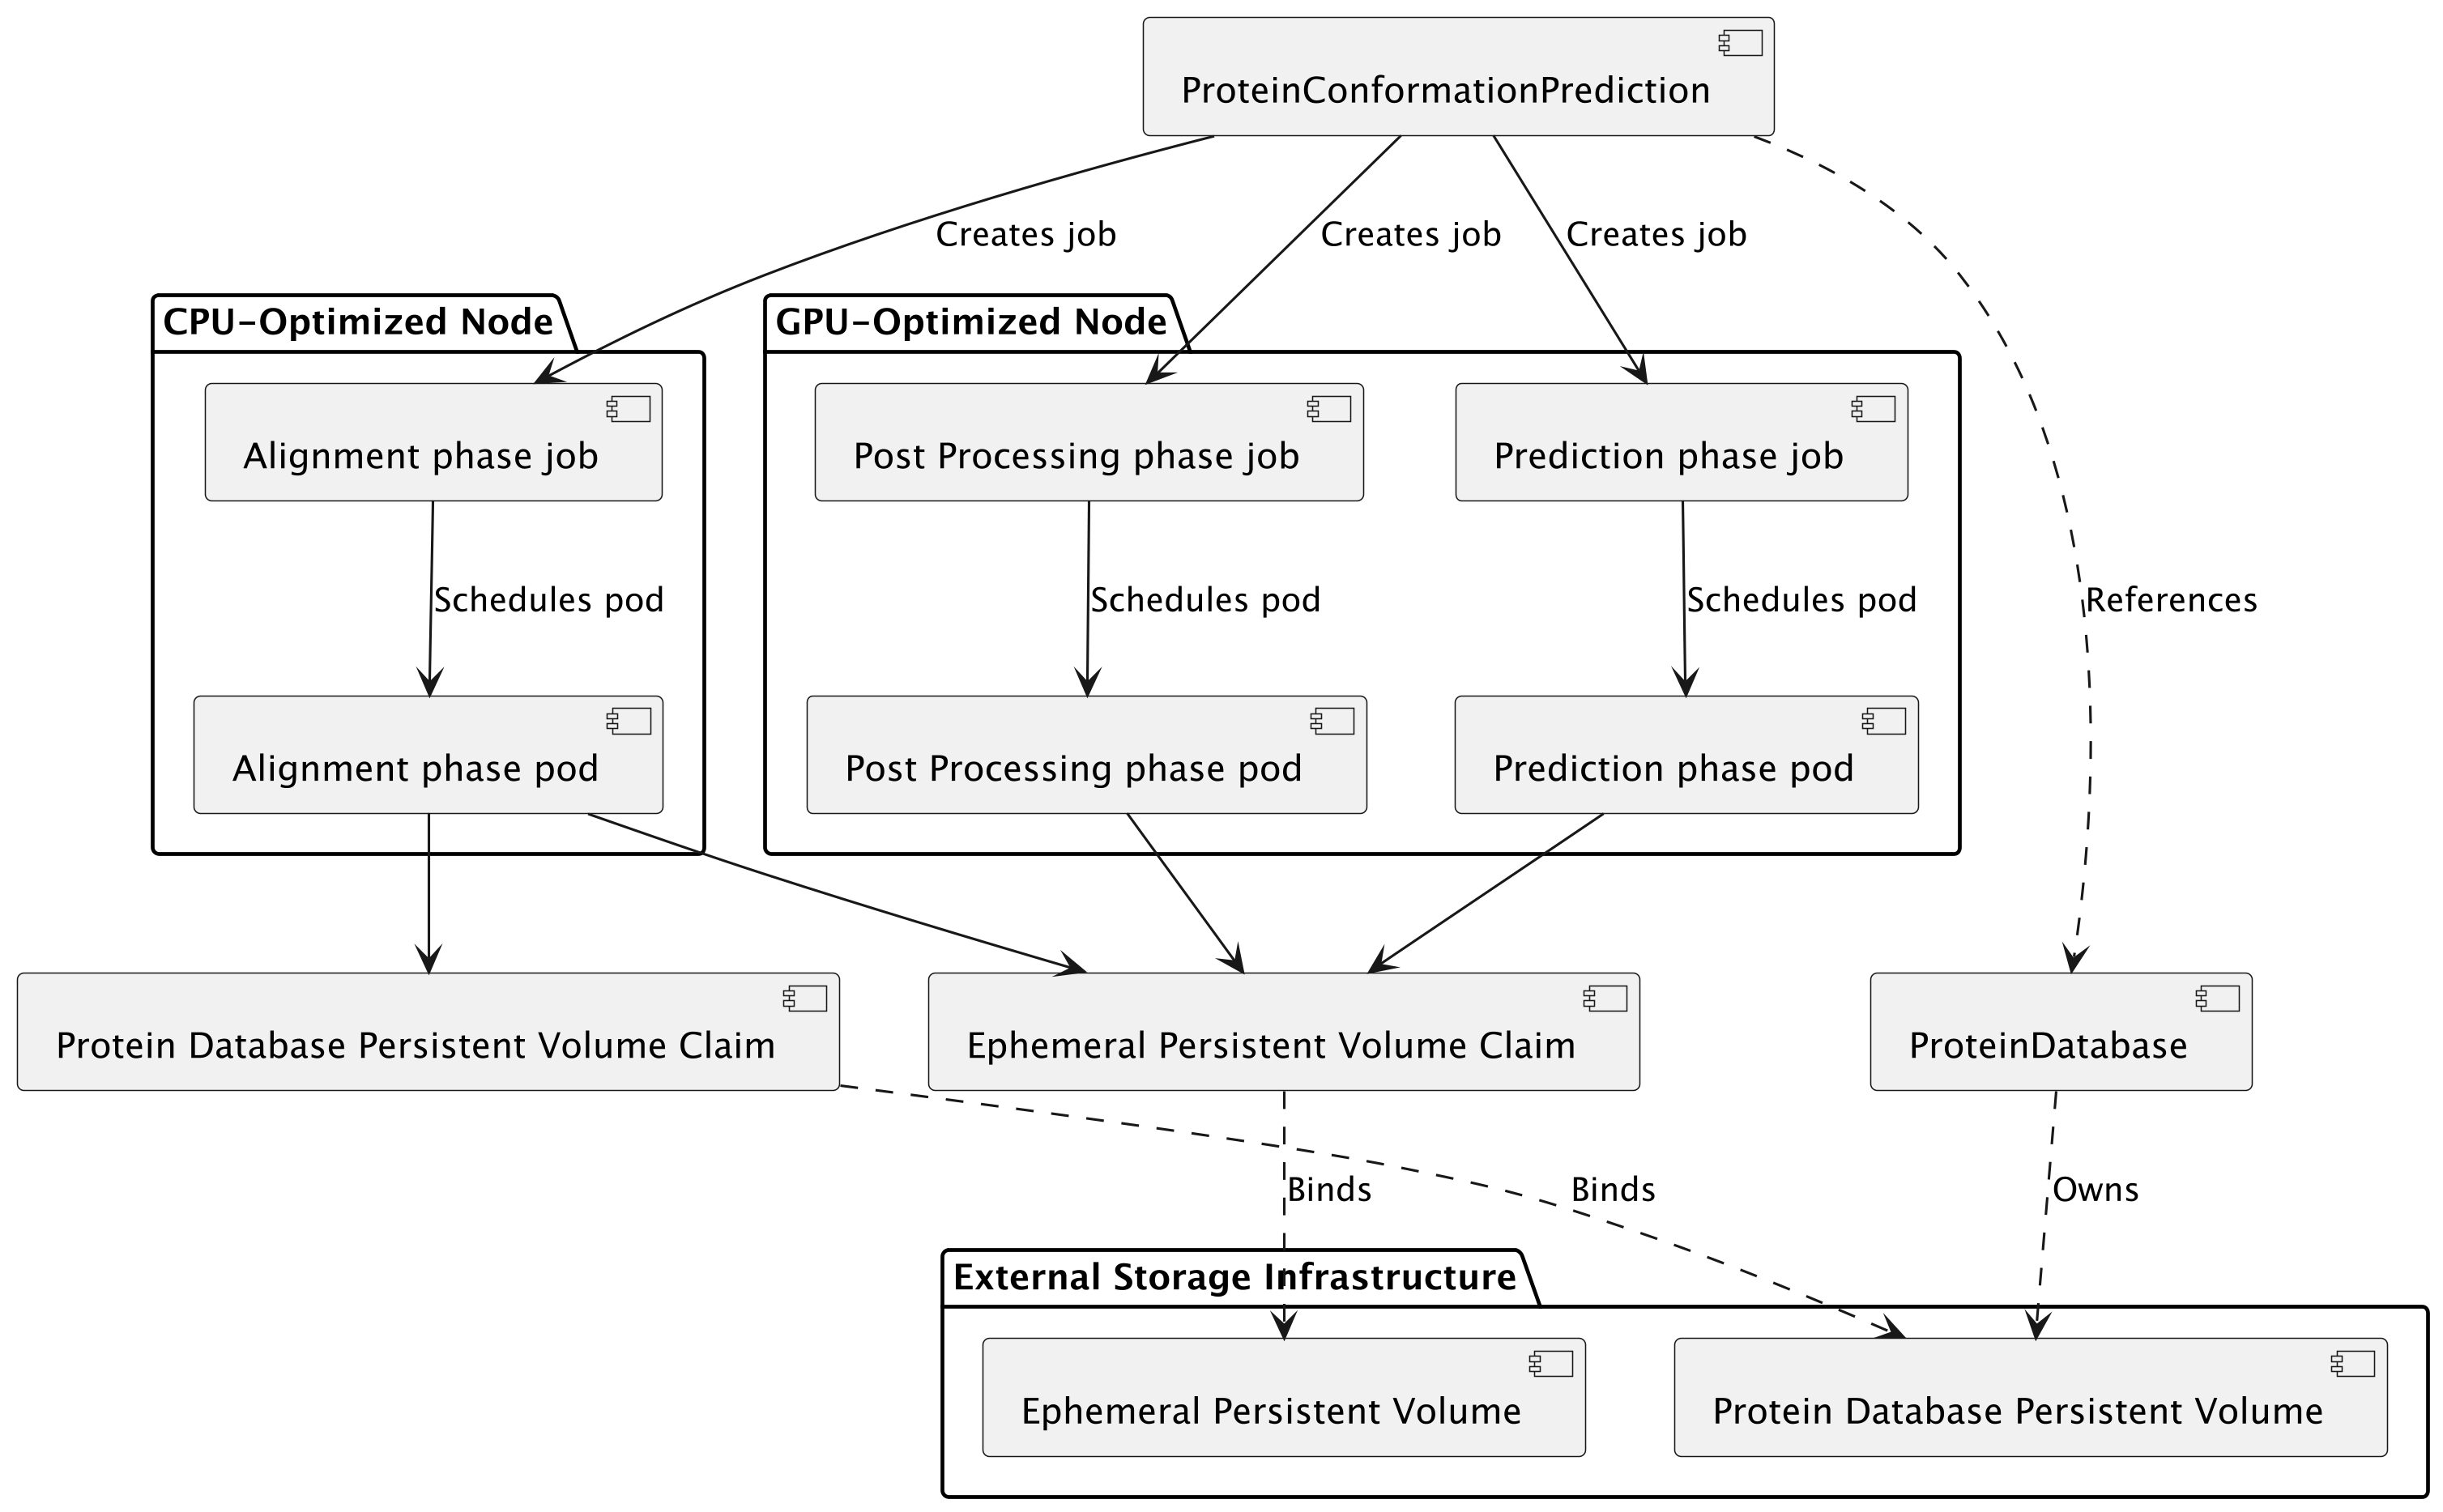
\includegraphics[width=\textwidth]{images/proteinconformationprediction}
    \caption{Cluster resource architecture of ProteinConformationPrediction}
    \label{fig:proteinconformationprediction}
\end{figure}

On the other hand, the \texttt{ProteinConformationPrediction} resource manages three jobs.
\begin{itemize}
    \item Alignment Phase.
    In this phase, AlphaFold searches existing protein databases to find matches.
    This phase takes place on scheduled instances optimized for CPU. The pod uses the AlphaFold image.
    \item Prediction Phase.
    This phase is when the algorithm performs the actual prediction of the three--dimensional structure of the protein.
    In this phase, pods are scheduled on instances equipped with tensor computing accelerators.
    The pod also uses the AlphaFold image.
    \item Post Processing Phase.
    This phase is responsible for sending computation artifacts to the destination data storage and optionally sending notifications to the research team members.
    The pod uses the \textit{manager} component image.
\end{itemize}

Therefore, each \texttt{ProteinConformationPrediction} instance corresponds to exactly three jobs and three pods.
In addition, \texttt{ProteinConformationPrediction} creates a \texttt{PersistentVolumeClaim} for temporary data.
In this volume, artifacts from the Alignment phase and potentially found protein structures are stored.

Table~\ref{tab:protein_prediction_components} summarizes all components created for a single protein structure prediction instance:

\begin{table}[htbp]
\centering
\caption{Components created for single protein structure prediction instance}
\label{tab:protein_prediction_components}
\small
\begin{tabular}{|l|l|p{2.2cm}|c|p{2.8cm}|}
\hline
\textbf{Phase} & \textbf{Component} & \textbf{Hardware Req.} & \textbf{Pods} & \textbf{Volume Access} \\
\hline
\textbf{Setup} & 
PVC & 
Storage & 
0 & 
Temp data \\
\hline
\textbf{1. Alignment} & 
Job + Pod + initContainer & 
CPU optimized & 
1 + init & 
DB vol. (R), Temp vol. (W) \\
\hline
\textbf{2. Prediction} & 
Job + Pod & 
GPU nodes & 
1 & 
Temp vol. (R/W) \\
\hline
\textbf{3. Post-proc.} & 
Job + Pod & 
Standard & 
1 & 
Temp vol. (R), S3 (W) \\
\hline
\textbf{Total} & 
1 PVC + 3 Jobs & 
Mixed & 
3 + init & 
2 Volumes + Cloud \\
\hline
\end{tabular}
\end{table}

Similarly to the \texttt{ProteinDatabase} resource, the resources are connected using the \textit{ownerReferences} mechanism.
The resource dependency architecture is shown in figure~\ref{fig:proteinconformationprediction}.


\section{Components overview}

\subsection{Kubernetes Operator}\label{subsec:component-operator}
\textit{Code repository: \url{https://github.com/kubefold/operator}}

The main component of the KubeFold platform written in Go.
The operator is installed on the Kubernetes cluster as a Deployment resource and connects to the Kubernetes API Server using the appropriate ClusterRole.
This gives it access to the REST API interface, which allows managing resources created within the cluster.

The most important elements of the KubeFold operator are two controllers, responsible for reconciling two CRD definitions introduced within the project.
Each cluster operator works on the infinite control loop, that constantly monitors changes in expected resource states in the cluster and adjusts the actual state to be as close as possible to the specified.
In the case of the KubeFold operator, the control loop works only on a single operator instance.
The election system provided by the KubeBuilder tool determines which running instance will be selected.

The first controller reconciles the \texttt{ProteinDatabase} resource.
In case of a new resource of this type appearing, the following operations are performed:
\begin{enumerate}
    \item Creates a new \textt{PersistentVolumeClaim} and sets the \texttt{storageClassName} parameter,
    \item When the \textt{PersistentVolumeClaim} is bound to a specific volume, it creates several jobs corresponding to downloading individual databases.
    Each pod has a mounted this \textt{PVC}.
    \item Starts a log observer -- a separate goroutine constantly monitoring job states, pod states, and reading logs from them.
    Thanks to the logs, it is able to dynamically update the \texttt{ProteinDatabase} status informing the user about the progress of downloading and also monitor the connection throughput.
\end{enumerate}
These operations are shown in figure~\ref{fig:proteindatabase_controller}.

\begin{figure}[htbp]
    \centering
    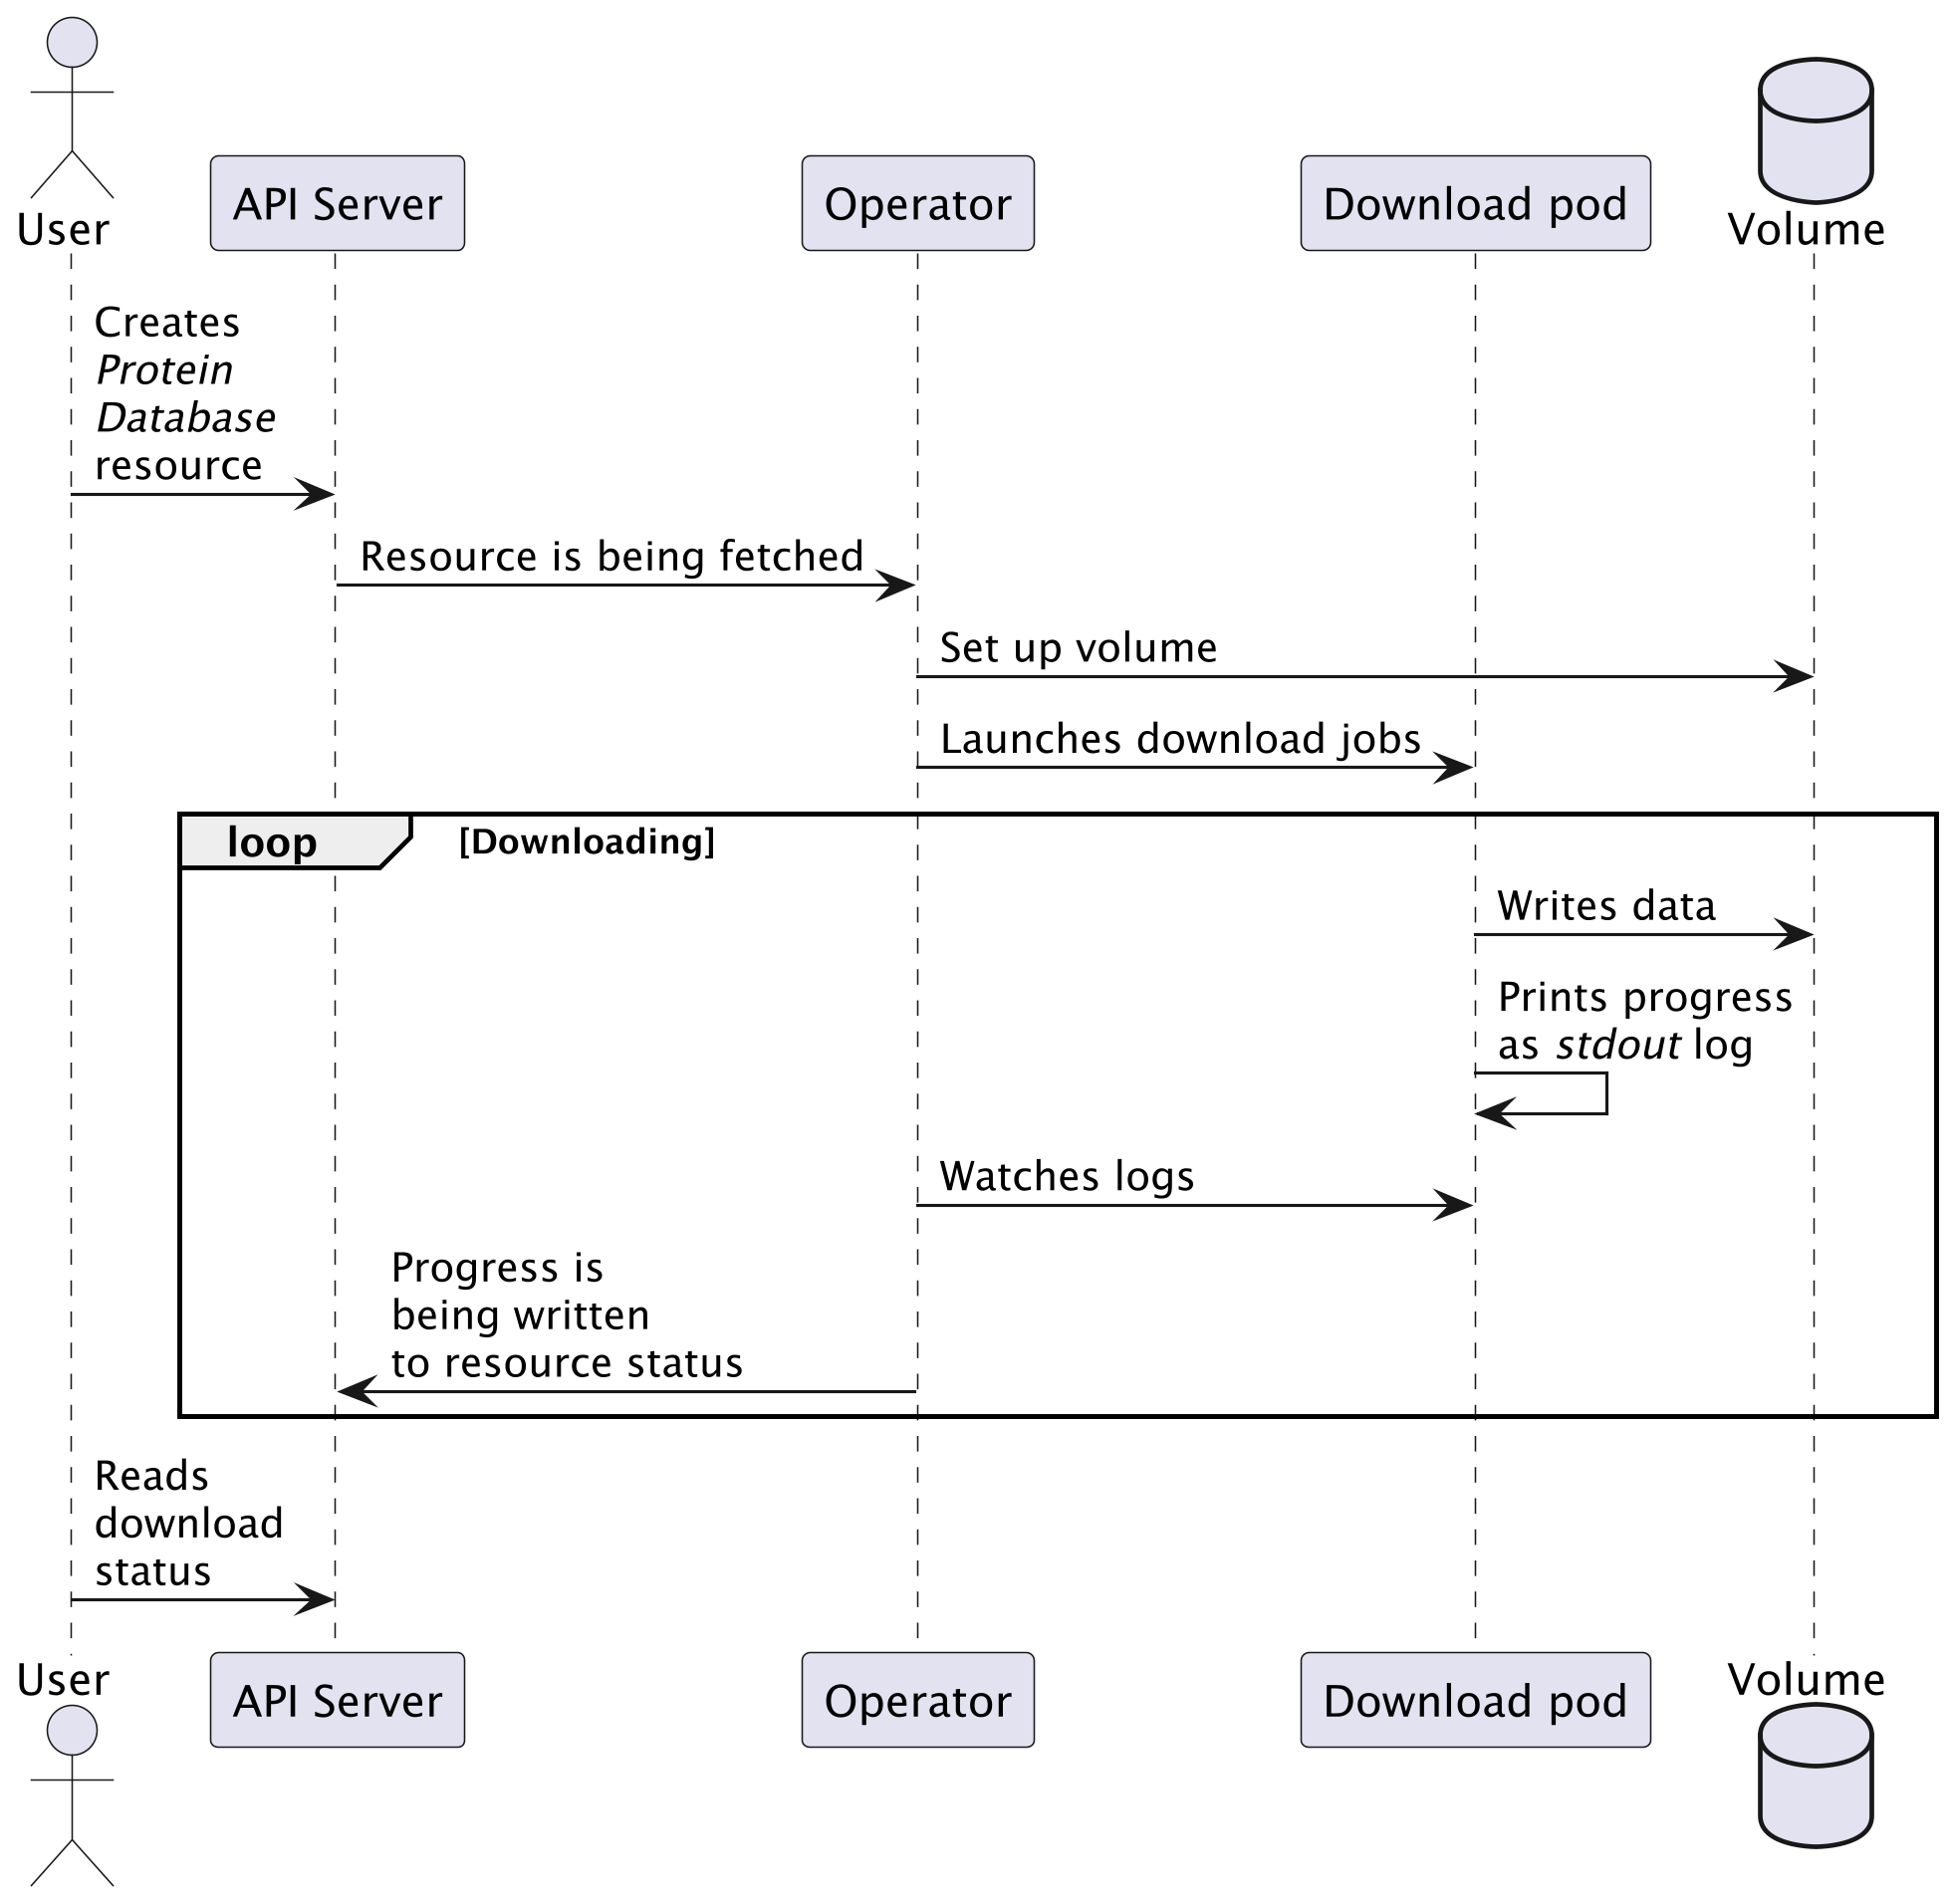
\includegraphics[width=\textwidth]{images/proteindatabase_controller}
    \caption{ProteinDatabase Controller behaviour}
    \label{fig:proteindatabase_controller}
\end{figure}

\begin{figure}[htbp]
    \centering
    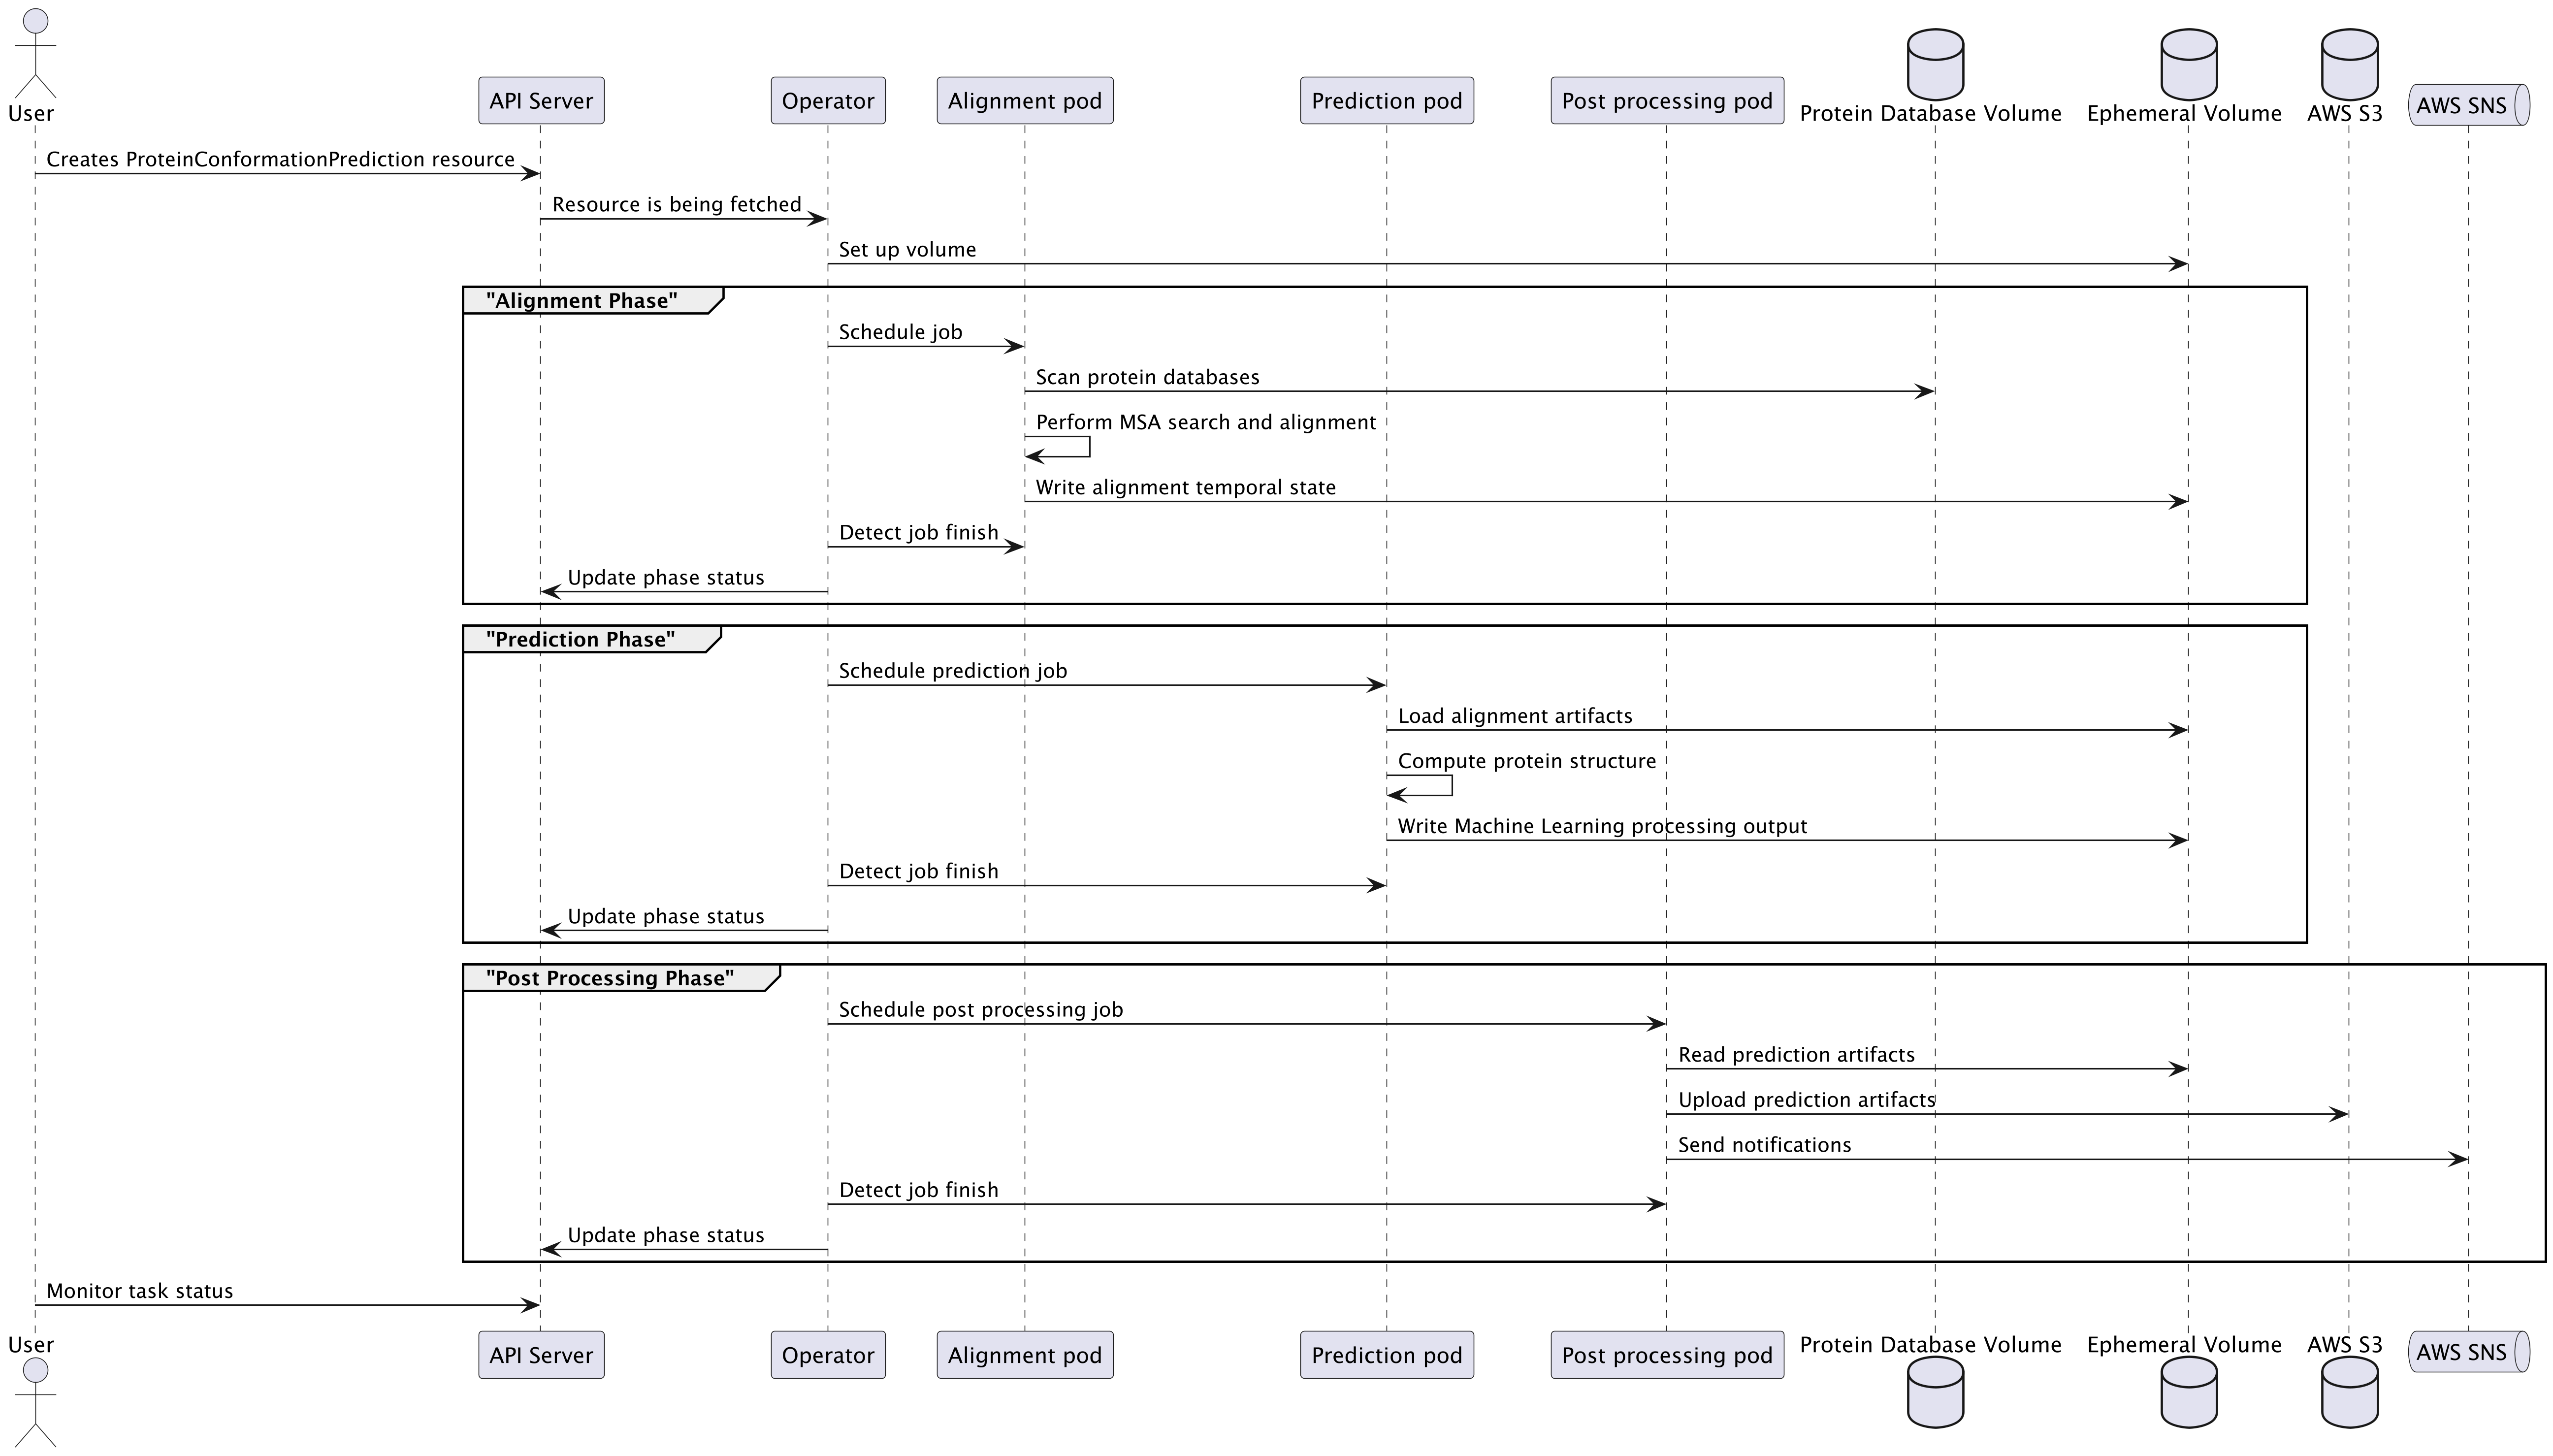
\includegraphics[width=0.9\textwidth]{images/proteinconformationprediction_controller}
    \caption{ProteinConformationPrediction Controller behaviour}
    \label{fig:proteinconformationprediction_controller}
\end{figure}

The second controller handles the \texttt{ProteinConformationPrediction} resource.
It contains the logic responsible for the three prediction phases of the protein structure.
The business logic (shown in figure~\ref{fig:proteinconformationprediction_controller}) after detecting a new resource performs the following steps:
\begin{enumerate}
    \item Creates a new \textit{PersistentVolumeClaim} for storing temporary program AlphaFold files,
    \item Starts a \textit{Job} that performs Alignment of the sequence and saves the state to the temporary volume.
    Also mounts the volume containing the protein databases.
    The AlphaFold program expects initial settings (for example sequence amino acids) as a JSON file named \texttt{fold\_input.json}.
    This file is created in this step using a special \textit{initContainer} ~\cite{k8s_init_containers}.
    The file content is prepared in the operator, then it is encoded to \texttt{base64} and injected into the init container via environment variables.
    The init container uses the \textit{manager} component image (described in~\ref{subsec:component-manager}).
    \item Starts a \textit{Job} corresponding to predicting the three--dimensional structure of the protein.
    The controller mounts the previously used volume, which contains the state from the alignment phase.
    This \textit{Job} has \textit{nodeAffinity} set so it can be scheduled on high--performance GPU nodes.
    \item Starts a \textit{Job} for post processing.
    This step loads computation artifacts and sends them to AWS S3. It also handles queuing notifications (e.g.\     SMS) for individual research team members.
\end{enumerate}

\subsection{Error Handling and Resilience}

The KubeFold operator implements comprehensive error handling mechanisms to ensure robustness and reliability of protein structure prediction workflows:

\begin{itemize}
    \item \textbf{Automatic Retry Mechanism} -- Each job phase (Alignment, Prediction, Post-processing) automatically retries up to 3 times in case of failure. 
    The operator tracks retry counts in the resource status and implements exponential backoff between attempts.
    
    \item \textbf{Timeout Management} -- Jobs have configurable timeouts with a default of 24 hours per phase. 
    If a job exceeds its timeout, the operator marks the prediction as failed and triggers cleanup procedures.
    
    \item \textbf{Failure Detection} -- The operator continuously monitors job status and immediately detects failures through Kubernetes job status indicators.
    Failed jobs are automatically deleted and recreated for retry attempts.
    
    \item \textbf{Resource Cleanup} -- In case of failures or completion, the operator automatically cleans up temporary resources including PersistentVolumeClaims and completed jobs to prevent resource leaks.
    
    \item \textbf{Event Recording} -- All significant events (job creation, failures, retries) are recorded as Kubernetes events, providing detailed audit trails for troubleshooting and monitoring.
    
    \item \textbf{Graceful Degradation} -- If critical dependencies (like ProteinDatabase) are unavailable, the operator enters a waiting state with periodic reconciliation rather than failing permanently.
    
    \item \textbf{Validation Guards} -- Input validation prevents invalid configurations from entering the processing pipeline, with detailed error messages returned to users.
\end{itemize}

This error handling approach ensures that transient failures (network issues, temporary resource unavailability) are automatically resolved, while permanent failures are clearly identified and reported to users through status updates and events.

\subsection{Downloader Component}\label{subsec:component-downloader}
\textit{Code repository: \url{https://github.com/kubefold/downloader}}

The \textit{downloader} component is responsible for downloading a single selected protein database.
Running this component in a container automatically starts download process.
The container expects the following environment variables to be configured:

\begin{itemize}
    \item \texttt{DATASET} -- the name of the dataset.
    The acceptable values of this variable are predefined.
    They are:
    \subitem \texttt{mgy\_clusters\_2022\_05.fa} -- MGY Clusters,
    \subitem \texttt{bfd-first\_non\_consensus\_sequences.fasta} -- BFD non--consensus sequences,
    \subitem \texttt{uniref90\_2022\_05.fa} -- UniRef90,
    \subitem \texttt{uniprot\_all\_2021\_04.fa} -- UniProt,
    \subitem \texttt{pdb\_2022\_09\_28\_mmcif\_files.tar} -- PDB mmCIF files,
    \subitem \texttt{pdb\_seqres\_2022\_09\_28.fasta} -- PDB sequence resources,
    \subitem \texttt{rnacentral\_active\_seq\_id\_90\_cov\_80\_linclust.fasta} -- RNACentral,
    \subitem \texttt{nt\_rna\_2023\_02\_23\_clust\_seq\_id\_90\_cov\_80\_rep\_seq.fasta} -- NT RNA,
    \subitem \texttt{rfam\_14\_9\_clust\_seq\_id\_90\_cov\_80\_rep\_seq.fasta} -- RFam,
    \item \texttt{DESTINATION} -- the path to the output directory,
    \item \texttt{RATE} (optional) -- the download speed limit expressed in kilobytes per second.
    The default process download does not have an upper limit set.
\end{itemize}.

All databases are hosted in the Google Cloud Storage service.
Almost all of them are \textit{.fasta}~\cite{pearson1988fasta} files compressed with the \textit{ZStandard} (or shorter \textit{zstd}) algorithm from Facebook~\cite{zstandard}.
The exception is the \texttt{pdb\_2022\_09\_28\_mmcif\_files.tar} file, which is a TAR archive (also compressed with \textit{zstd}).

The component downloads and decompresses files at the same time.
Every few moments, a separate goroutine monitors the progress of already downloaded data and outputs to \texttt{stdout} a logline with the current state.
A sample logline is shown in listing~\ref{lst:downloader_logline}.
Thanks to this, the operator can read download progress and update the \texttt{ProteinDatabase} status.
After successful completion or interrupted download, the process exits logging the valid message to logs and returning the appropriate exit code.

\begin{lstlisting}[language=txt,caption={Sample logline from downloader},label={lst:downloader_logline}]
{"dataset":"rnacentral_active_seq_id_90_cov_80_linclust.fasta","level":"info","msg":"Download progress","size":7700349721,"time":"2025-05-17T16:53:52+02:00","total":13860314914,"type":"download","unit":"bytes"}
\end{lstlisting}

\subsection{Manager Component}\label{subsec:component-manager}
\textit{Code repository: \url{https://github.com/kubefold/manager}}

The \textit{manager} component is responsible for three independent tasks:
\begin{itemize}
    \item configuring the \textt{fold\_input.json} file for the AlphaFold program,
    \item sending computation artifacts to the AWS S3 service (more about it in section~\ref{subsec:amazon-s3-object-storage}),
    \item queuing notifications using the AWS SNS / AWS End User Messaging service (more about it in section~\ref{subsec:amazon-sns}).
\end{itemize}

The selected operation depends on which environment variables are configured in the container.
For each operation, two environment variables are mandatory:
\begin{itemize}
    \item \texttt{INPUT\_PATH} -- the path to the AlphaFold data input directory,
    \item \texttt{OUTPUT\_PATH} -- the path to the AlphaFold data output directory.
\end{itemize}

To save the \textt{fold\_input.json} file, the \texttt{ENCODED\_INPUT} variable should be set, which should contain the encoded in \texttt{base64} JSON configuration.

To send artifacts, the \texttt{BUCKET} environment variable should be set to the S3 bucket path (full URL, including \textt{s3:\/\/}).
To send a notification using the AWS End User Messaging service, the container must have the \texttt{NOTIFICATION\_PHONES} and \texttt{NOTIFICATION\_MESSAGE} variables set.
The variable with phone numbers can contain more than one recipient -- in such a case, phone numbers should be provided as a comma--separated list.

If using AWS services, the AWS client variables should be configured.
This can be done using environment variables such as \texttt{AWS\_ACCESS\_KEY\_ID} and \texttt{AWS\_SECRET\_ACCESS\_KEY}.
An alternative is to configure the AWS IAM role to be used by the container and have access permissions to the individual services.
    %1. Describe EKS cluster
%2. Describe how was operator installed (screenshots etc)
%3. Describe prepared CRD
%4. Describe execution (screenshots)
%5. Describe artifacts
%6. Show SMS

\chapter{Methods and Experiments}

Niniejszy rozdział ma za zadanie opisać sposób testowania oprogramowania KubeFold na platformie AWS oraz omówi wyniki obliczeń.


\section{Runtime environment}

Projekt był uruchamiany na platformie AWS EKS~\ref{subsec:aws-eks}.
Do szybkiego uruchomienia klastra użyto narzędzia \texttt{eksctl}, któremu podano konfigurację klastra w regionie \texttt{eu-central-1} z dwiema grupami węzłów-CPU i GPU.
Konfiguracja została przedstawiona na listingu~\ref{lst:eksctl}.
Warto zwrócić uwagę na dołączone polityki AWS IAM dające uprawnienia grupom węzłów do usług takich jak AWS S3, AWS SNS czy też AWS FSx.

\begin{lstlisting}[language=yaml,caption={\texttt{eksctl} configuration used for launching AWS EKS cluster},label={lst:eksctl}]
apiVersion: eksctl.io/v1alpha5
kind: ClusterConfig
metadata:
  name: alphafold-cluster
  region: eu-central-1

managedNodeGroups:
  - name: ng-primary # Cheaper node group without GPU devices
    instanceType: m5.xlarge
    desiredCapacity: 1
    subnets:
      - "subnet-038b10f6f4ac5aacd"
    iam:
      withAddonPolicies:
        ebs: true
        fsx: true
        efs: true
      attachPolicyARNs:
        - arn:aws:iam::aws:policy/AmazonEKSWorkerNodePolicy
        - arn:aws:iam::aws:policy/AmazonEKS_CNI_Policy
        - arn:aws:iam::aws:policy/AmazonFSxFullAccess
        - arn:aws:iam::aws:policy/AmazonS3FullAccess
        - arn:aws:iam::aws:policy/AmazonSNSFullAccess
        - arn:aws:iam::aws:policy/AmazonEC2ContainerRegistryReadOnly
        - arn:aws:iam::aws:policy/AmazonSSMManagedInstanceCore
  - name: ng-gpu # More expensive node group with GPU devices
    instanceType: g5.xlarge
    desiredCapacity: 1
    subnets:
      - "subnet-038b10f6f4ac5aacd"
    iam:
      withAddonPolicies:
        ebs: true
        fsx: true
        efs: true
      attachPolicyARNs:
        - arn:aws:iam::aws:policy/AmazonEKSWorkerNodePolicy
        - arn:aws:iam::aws:policy/AmazonEKS_CNI_Policy
        - arn:aws:iam::aws:policy/AmazonFSxFullAccess
        - arn:aws:iam::aws:policy/AmazonS3FullAccess
        - arn:aws:iam::aws:policy/AmazonSNSFullAccess
        - arn:aws:iam::aws:policy/AmazonEC2ContainerRegistryReadOnly
        - arn:aws:iam::aws:policy/AmazonSSMManagedInstanceCore

iam:
  withOIDC: true
  serviceAccounts:
    - metadata:
        name: fsx-csi-controller-sa
        namespace: kube-system
        labels: { aws-usage: "application" }
      attachPolicyARNs:
        - "arn:aws:iam::aws:policy/AmazonFSxFullAccess"

vpc:
  id: vpc-0ade33da149682ec2
  subnets:
    public:
      eu-central-1a:
        id: "subnet-038b10f6f4ac5aacd"
      eu-central-1b:
        id: "subnet-099b2b55ca156bb7d"

addons:
  - name: vpc-cni
  - name: coredns
  - name: kube-proxy
  - name: eks-pod-identity-agent
\end{lstlisting}

Na klastrze został zainstalowany AWS FSx CSI Driver.
Służy on do automatycznego tworzenia i zarządzania wolumenami AWS FSx for Lustre na postawie utworzonych w klastrze zasobów \texttt{PersistentVolumeClaim}.
By było to możliwe koniecznie jest skonfigurować \texttt{StorageClass}, która wskazuje w jaki sposób powinny być utworzone wolumeny.
W konfiguracji przedstawionej na listingu~\ref{lst:storage-class} ustawiono opcje takie jak wersja systemu plików, typ kompresji (disabled), przepustowość wolumenu oraz opcje sieciowe.
Dzięki temu utworzenie zasobu \texttt{PersistentVolumeClaim} ze wskazaniem na \texttt{StorageClass} o nazwie \texttt{fsx-sc} spowoduje automatycznie provisioning nowego wolumenu w AWS.

\begin{lstlisting}[language=yaml,caption={Definition of \texttt{StorageClass} for FSx CSI Driver},label={lst:storage-class}]
kind: StorageClass
apiVersion: storage.k8s.io/v1
metadata:
  name: fsx-sc
provisioner: fsx.csi.aws.com
parameters:
  subnetId: subnet-038b10f6f4ac5aacd
  securityGroupIds: sg-058c31d84bfd004cf,sg-04e79090b86912eae,sg-07d7ceb3fa050568c,sg-02a2a067c7f724318
  deploymentType: PERSISTENT_1
  perUnitStorageThroughput: "200"
  dataCompressionType: "NONE"
  fileSystemTypeVersion: "2.15"
\end{lstlisting}

Do zainstalowania operatora KubeFold użyto pliku instalacyjnego wygenerowanego przez narzędzie KubeFold.
Znajduje się on w repozytorium kodu w serwisie GitHub w ścieżce \texttt{dist/install.yaml}.
Instalacja zatem sprowadza się do wykonania jednego polecenia: \texttt{kubectl apply -f https://raw.githubusercontent.com/kubefold/operator/ \n refs/heads/main/dist/install.yaml}.
Dzięki temu jest ona bardzo szybka i wygodna z perspektywy administratora.

\begin{lstlisting}[language=bash,caption={Quick project startup script},label={lst:up-script}]
#!/bin/bash

export AWS_PAGER=""
ACCOUNT_ID=$(aws sts get-caller-identity --query Account --output text)
eksctl create cluster -f eks/cluster.yaml
aws eks update-kubeconfig --name alphafold-cluster --region eu-central-1
kubectl config use-context arn:aws:eks:eu-central-1:"$ACCOUNT_ID":cluster/alphafold-cluster
kubectl apply -k "github.com/kubernetes-sigs/aws-fsx-csi-driver/deploy/kubernetes/overlays/stable/?ref=release-1.3"
kubectl apply -f eks/fsx.storageclass.k8s.yaml

kubectl apply -f https://raw.githubusercontent.com/kubefold/operator/refs/heads/main/dist/install.yaml
kubectl apply -f config/samples/data_v1_proteindatabase.yaml

echo 'Done'
\end{lstlisting}

W celu szybkiego postawienia klastra wraz ze wszystkimi potrzebnymi zależnościami został przygotowany skrypt \texttt{up.sh}, który został przedstawiony na listingu~\ref{lst:up-script}.
Po wykonaniu skryptu można bezpośrednio przejść do rozpoczęcia pracy z KubeFold.
Jeżeli klaster został zainstalowany poprawnie, wykonanie polecenia \texttt{kubectl get pods -A} powinno pokazać wyjście podobne do tego na zrzucie ekranu~\ref{fig:eks_pods_terminal}.

\begin{figure}[htbp]
  \centering
  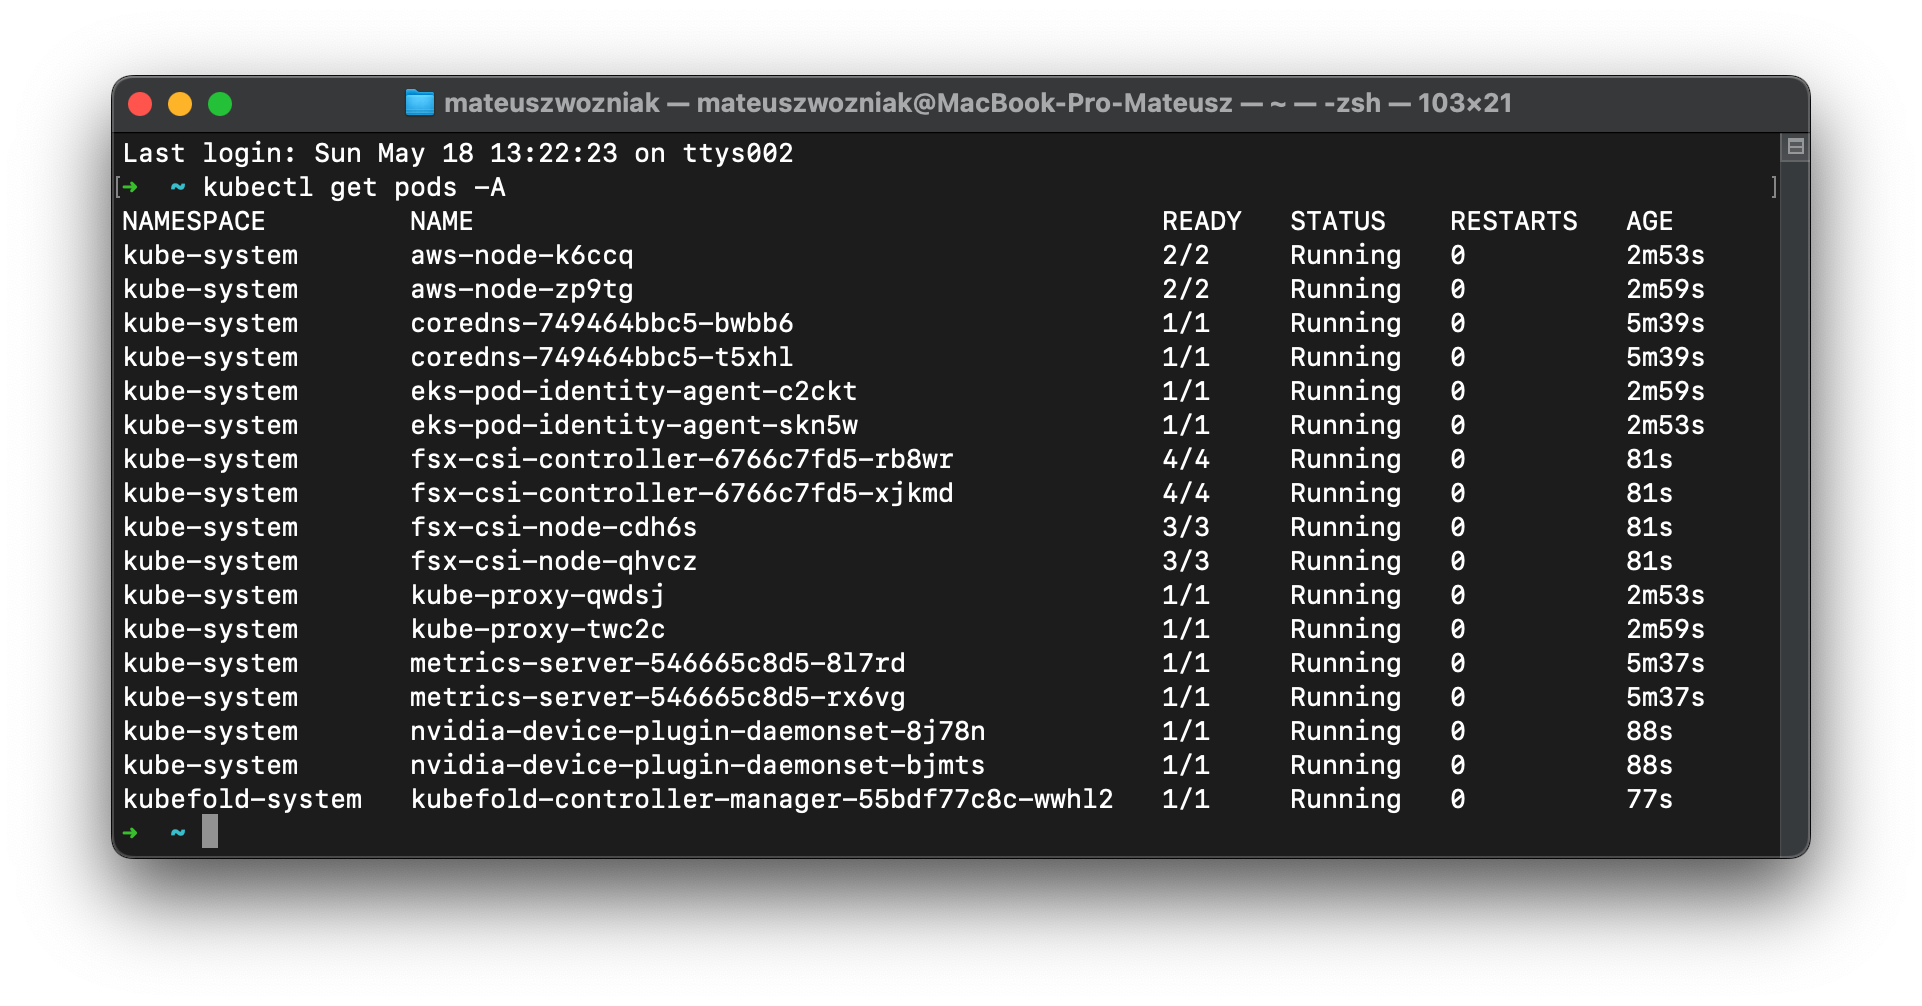
\includegraphics[width=\textwidth]{images/eks_pods_terminal}
  \caption{\texttt{kubectl get pods} output after successful cluster installation}
  \label{fig:eks_pods_terminal}
\end{figure}


\section{Prepared resource definitions}

W celu przeprowadzenia testów KubeFold przygotowano następujące definicje zasobów w kodzie YAML.
Pierwszy z nich to zasób \texttt{ProteinDatabase} przedstawiony na listingu~\ref{lst:used_protein_database}.
Drugi z nich z kolei to zasób \texttt{ProteinConformationPrediction} przedstawiony na listingu~\ref{lst:used_protein_conformation_prediction}.
Oba te zasoby zostały zaaplikowane na klaster za pomocą \texttt{kubectl apply} tuż po instalacji.

\begin{lstlisting}[language=yaml,caption={Used \texttt{ProteinDatabase} resource definition},label={lst:used_protein_database}]
apiVersion: data.kubefold.io/v1
kind: ProteinDatabase
metadata:
  name: proteindatabase-sample
spec:
  datasets:
    bfd: true
    mgyclusters: true
    nt: true
    pdb: true
    pdbseqreq: true
    rfam: true
    rnacentral: true
    uniref90: true
    uniprot: true
  volume:
    storageClassName: fsx-sc
\end{lstlisting}

\begin{lstlisting}[language=yaml,caption={Used \texttt{ProteinConformationPrediction} resource definition},label={lst:used_protein_conformation_prediction}]
apiVersion: data.kubefold.io/v1
kind: ProteinConformationPrediction
metadata:
  name: proteinconformationprediction-sample
spec:
  database: proteindatabase-sample
  protein:
    id: [ 'A','B' ]
    sequence: GMRESY...LQQANDLKQG
  model:
    volume:
      storageClassName: fsx-sc
    weights:
      http: https://staticfilehosting.com/af3.bin.zst
    seeds:
      - 1
  destination:
    s3:
      bucket: kubefold-artifacts-sample
      region: eu-central-1
  notify:
    region: eu-central-1
    sms:
      - "+48140690323"
\end{lstlisting}.

Po utworzeniu zasobu \texttt{ProteinDatabase} FSx CSI Driver spowodował utworzenie systemu plików FSx for Lustre (zobacz rys.~\ref{fig:fsx_fs}).
Gdy tylko system plików został utworzony, proces pobierania baz danych białek rozpoczął się w wielu podach jednocześnie.
Użytkownik może na bieżąco kontrolować postęp pobierania co zostało pokazane na zrzucie ekranu~\ref{fig:used_proteindatabase_terminal}.

\begin{figure}[htbp]
  \centering
  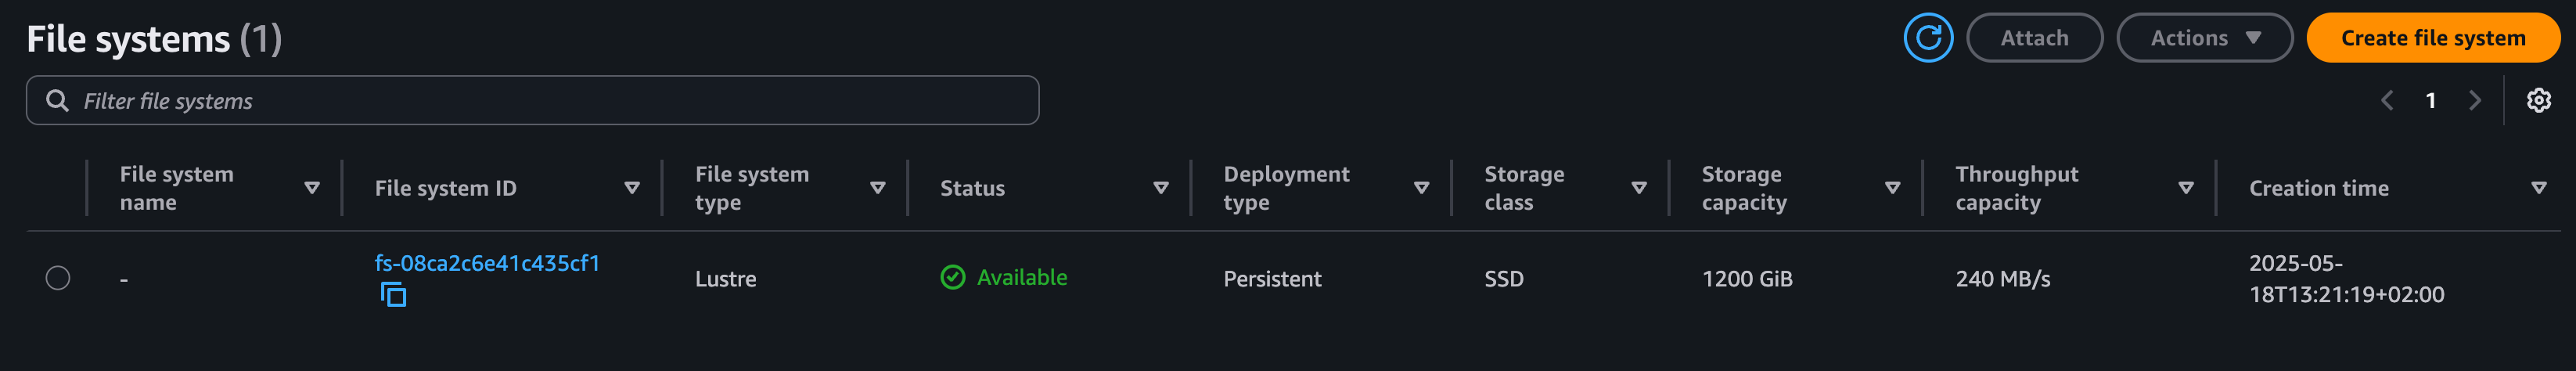
\includegraphics[width=\textwidth]{images/fsx_fs}
  \caption{Created FSx for Lustre file system in AWS Web Console}
  \label{fig:fsx_fs}
\end{figure}

\begin{figure}[htbp]
  \centering
  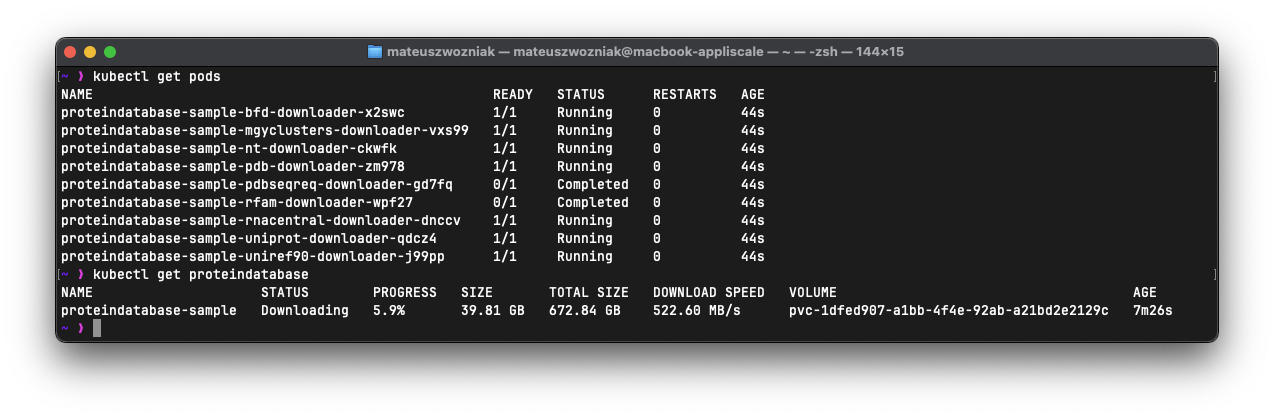
\includegraphics[width=\textwidth]{images/old_proteindatabase_terminal}
  \caption{Terminal output presenting \texttt{ProteinDatabase} resource}
  \label{fig:used_proteindatabase_terminal}
\end{figure}

\section{Computation artifacts overview}
    \chapter{Results}

\section{Implementation of the KubeFold Project}

Within the project, the following goals were successfully accomplished:
\begin{itemize}
    \item Designed and implemented the \textit{KubeFold} operator for the Kubernetes platform.
    \item Created two custom resources (CRDs):
    \begin{itemize}
        \item \textit{ProteinDatabase} – managing protein databases,
        \item \textit{ProteinConformationPrediction} – running protein conformation prediction computations.
    \end{itemize}
    \item Developed a component for automatic downloading and decompression of protein databases.
    \item Prepared infrastructure as code (IaC) allowing for quick operator deployment in AWS cloud (EKS + FSx for Lustre).
    \item Created documentation and installation instructions for the Kubernetes operator.
    \item Conducted several protein conformation computations to test the solution.
\end{itemize}


\section{Comparison of Other Solutions}

The AlphaFold algorithm has significantly influenced the development of bioinformatics, offering breakthrough capabilities in predicting protein spatial structures.
However, its practical use comes with significant computational and technological requirements.
In response to these challenges, alternative solutions have emerged, such as \textbf{OpenFold}\cite{openfold} and \textbf{ColabFold}\cite{colabfold}, which aimed to simplify the prediction process and increase its accessibility.
However, \textbf{KubeFold} – the system developed as part of this work – stands out among these tools, providing a much higher level of automation, scalability, and cloud infrastructure integration.

\subsection*{OpenFold}

OpenFold is an open-source reimplementation of AlphaFold2, written in Python using the PyTorch library.
This project is primarily targeted at research teams and institutions that have extensive computational infrastructure and need full control over the prediction process.
OpenFold enables, among other things, training models from scratch, testing architecture modifications, and running tasks in distributed environments (HPC, cloud).

Due to the advanced nature of the tool, its implementation requires high expertise in machine learning, container management, and cloud environment configuration.
Significant hardware resources (e.g., A100-class GPU cards) are also necessary, which may be an entry barrier for smaller teams.

\subsection*{ColabFold}

ColabFold is a simplified version of AlphaFold2, available through interactive notebooks running in the Google Colaboratory environment.
Thanks to integration with the MMseqs2 tool, the sequence alignment process is much faster, and users don't need to configure the environment or install software themselves.

ColabFold is primarily aimed at individuals and teams that don't have advanced computational infrastructure.
Despite the low entry threshold, this solution has numerous limitations: it doesn't allow model training, is dependent on Colab platform limitations (session time, GPU availability), and its application is mainly limited to simple, single predictive tasks.

\subsection*{Advantages of the KubeFold Approach}

The \textbf{KubeFold} platform developed as part of this work represents a modern and flexible alternative to the above solutions.
By utilizing Kubernetes technology and integration with Amazon Web Services (such as FSx for Lustre and S3), KubeFold automates the entire process of running protein conformation predictions – from downloading databases, through running calculations, to archiving results and sending notifications.

Unlike OpenFold, KubeFold doesn't require manual task configuration or infrastructure management – all components are automatically launched based on YAML resources, which significantly simplifies the process.
Compared to ColabFold, the KubeFold platform offers much greater scalability and control over computational resources – allowing for simultaneous running of multiple tasks and allocating appropriate resources (CPU, GPU, memory, disk space).

This approach combines the advantages of flexibility and computational power with ease of use, making KubeFold a more comprehensive solution adapted to the real needs of research environments and production applications.

A detailed comparison of the computational infrastructure for OpenFold, ColabFold, and KubeFold is presented in Table~\ref{tab:comparison}.

\begin{table}[H]
    \centering
    \small
    \begin{tabularx}{\textwidth}{|X|X|X|X|}
        \hline
        \textbf{Features}                           & \textbf{OpenFold}                         & \textbf{ColabFold}                & \textbf{KubeFold (proposed)}                          \\
        \hline
        \textbf{Platform}                           & HPC clusters, cloud (AWS, GCP)            & Google Colab, local environments & Kubernetes + AWS EKS \\
        \hline
        \textbf{Hardware requirements}              & High (GPU A100, RAM 64GB+)                & Low (free GPU in Colab) & Medium-high, dynamically scalable \\
        \hline
        \textbf{Automation}                         & Manual task and environment configuration & None, manual handling by user & Full automation through Kubernetes operator \\
        \hline
        \textbf{Scalability}                        & High, but difficult to configure          & Limited to single predictions & Very high, supports parallel processing \\
        \hline
        \textbf{Ease of deployment}                 & High entry threshold (DevOps, ML)         & Very easy, suitable for beginners & Medium threshold, requires basic Kubernetes knowledge \\
        \hline
        \textbf{Integration with external services} & Requires own implementation               & None                              & Yes – AWS S3, FSx, SNS, IAM                           \\
        \hline
    \end{tabularx}
    \caption{Comparison of computational infrastructure: OpenFold, ColabFold, and KubeFold}
    \label{tab:comparison}
\end{table}

\section{Challenges}

Głównym wyzwaniem było opracowanie odpowiedniej architektury platformy KubeFold, która jest w stanie działać na wielu węzłach klastra jednocześnie, optymalizując koszta i szybkość obliczeń.
Dzięki podziale procesu pobierania na wiele podów udało się zwiększyć potencajną szybkość pobierania baz danych białek.
Z kolei rozdział fazy \textit{Aligning} i \textit{Predicting} pozwolił optymalnie zutylizować zasoby obliczeniowe CPU i GPU.
Taki setup pozwala na zaoszczędzenie wydatków w chmurze publicznej.

Drugim wyzwaniem była odpowiednia implementacja komponentu \textit{downloader}.
Komponent ten musi w tym samym czasie pobierać jak i dekompresować dane.
Gdyby ten proces odbywał się sekwencyjnie, to chwilowo używana przestrzeń dyskowa byłaby dużo większa niż faktyczny rozmiar bazy danych.

Trzecim wyzwaniem było odpowiednie utworzenie infrastruktury do testowania platformy KubeFold.
Projekt uruchamia się korzystając z wielu usług chmury AWS, a to wymaga przemyślanego połączenia każdego komponentu.
Ustawienie odpowiednich ustawień subnetów, VPC czy driverów CSI wymagało poświęcenia sporej ilości czasu.


\section{Conclusions}
    %! suppress = MissingLabel
\chapter{Summary}

Within the project, the following goals were successfully accomplished:
\begin{itemize}
    \item Designed and implemented the \textit{KubeFold} operator for the Kubernetes platform.
    \item Created two custom resources (CRDs):
    \begin{itemize}
        \item \textit{ProteinDatabase} – managing protein databases,
        \item \textit{ProteinConformationPrediction} – running protein conformation prediction computations.
    \end{itemize}
    \item Developed a component for automatic downloading and decompression of protein databases,
    \item Prepared infrastructure as code (IaC) allowing for quick operator deployment in AWS cloud (EKS + FSx for Lustre),
    \item Created documentation and installation instructions for the Kubernetes operator,
    \item Conducted several protein conformation computations to test the solution.
\end{itemize}


\section{Project development possibilities}

The KubeFold platform presents several promising opportunities for future development.
Based on the current implementation and analysis, the following areas show particular potential for expansion:

\subsection{Resource optimization}
The platform's resource management capabilities could be enhanced through:
\begin{itemize}
    \item Smart scaling systems that predict and adapt to computation patterns,
    \item Advanced algorithms for optimizing cloud resource costs,
    \item Comprehensive analytics for resource usage and optimization.
\end{itemize}

\subsection{Bioinformatics workflow integration}
Expanding KubeFold's capabilities beyond AlphaFold would make it more versatile:
\begin{itemize}
    \item Supporting additional protein structure prediction algorithms,
    \item Enabling protein--protein interaction analysis,
    \item Adding automated validation tools for prediction results.
\end{itemize}

\subsection{User interface and experience}
Improving the platform's accessibility and usability through:
\begin{itemize}
    \item A modern web interface for managing and monitoring predictions,
    \item A comprehensive REST API for automated workflows,
    \item Interactive visualization tools for real--time progress tracking,
    \item Features supporting team collaboration and research workflows.
\end{itemize}
%
%\section{Conclusion}
%
%The development of KubeFold represents a significant step forward in making advanced protein structure prediction more accessible and manageable.
%The project demonstrates how modern cloud--native technologies can be effectively applied to complex scientific computing challenges.
%Looking ahead, the platform's architecture provides a solid foundation for future enhancements and integrations.
%
%KubeFold highlights the importance of combining domain expertise in bioinformatics with modern software engineering practices.
%The use of Kubernetes operators and cloud--native patterns has proven particularly effective in managing complex computational workflows.
%This approach could serve as a template for other scientific computing applications that require similar levels of automation and scalability.
%
%The project's impact extends beyond its immediate application in protein structure prediction.
%It showcases how cloud technologies can democratize access to advanced computational resources, potentially accelerating research in structural biology and related fields.
%The modular design and clear separation of concerns make it possible for other researchers and developers to build upon this work.
%The future of computational biology increasingly depends on scalable, automated solutions that can handle growing data volumes and computational demands.
%KubeFold's contribution to this field demonstrates how modern software engineering principles can be applied to create robust, maintainable, and scalable scientific computing platforms.

    \printbibliography

\end{document}